\documentclass[11pt]{article}

\usepackage[margin=1.1in]{geometry}
\usepackage{amsmath,amssymb}
\usepackage{graphicx}
\usepackage{booktabs}
\usepackage{multirow}
\usepackage{threeparttable}
\usepackage{setspace}
\usepackage[round]{natbib}
\usepackage[hidelinks]{hyperref}
\usepackage{caption}
\captionsetup{font=small,labelfont=bf}
\usepackage{enumitem}
\setstretch{1.15}
\emergencystretch=1.5em
% The PNG chart exhibits (pq_timing_overlay.png, pq_exact_timing.png, pq_model_stability.png,
% trading_dashboard2.png) sit NEXT TO this .tex file; for Overleaf, upload those PNGs alongside
% the .tex (the fig_*.pdf placeholders resolve from figures/).
\graphicspath{{./}{figures/}}

\newcommand{\pending}{\multicolumn{1}{c}{\textit{pending}}}
\newcommand{\Q}{\mathbb{Q}}
\newcommand{\PP}{\mathbb{P}}

\title{EVT Tails on a Neural Quantile Body:\\
Calibrated Multi-Horizon Return Distributions\\
and the Price of Crash Insurance\thanks{Working paper, first draft July 2026. Draft v2, July 2026 --- revised scope. Comments welcome. All results are from walk-forward experiments described in Section~\ref{sec:validation}; a live out-of-sample holdout beginning July 2026 is running at the time of writing. Economic results in Appendix~\ref{app:trading} use a placeholder transaction-cost assumption (10\% of premium) pending integration of measured OptionMetrics spreads; see Section~\ref{sec:limitations} and Appendix~\ref{app:costs}. A companion paper develops the residual-hybrid risk engine, the misspecification frontier, and generative-Bayesian extensions on broader universes; the two papers cross-reference and do not duplicate claims.}}
\author{Sean Qin}
\date{July 2026 --- Draft v2 (revised scope)}

\begin{document}

\maketitle

\begin{abstract}
\noindent We train a single horizon-conditioned implicit quantile network (IQN) that outputs the full term structure of conditional return distributions---horizons of one week to three months---for roughly 543 liquid US single names over 2005--2026. Out of sample, under an annual walk-forward protocol with a 95-day purge and embargo, the distribution body and upper tail are essentially exactly calibrated at every horizon (empirical coverage 0.486--0.492 at $\tau=0.50$, 0.693--0.699 at $\tau=0.75$, 0.898--0.900 at $\tau=0.95$), while the left tail is roughly twice too narrow: the 5\% quantile is breached about 10\% of the time. Heavier left-tail quantile sampling does not repair it (breach rate 0.108 versus 0.103), indicating an informational rather than architectural limit: crash-sized moves are driven by discrete idiosyncratic events not recoverable from price-based conditioning information. Grafting a generalized Pareto tail onto the neural quantile body, estimated strictly on past data within the walk-forward, restores calibration (5\% coverage 0.056--0.063 and 1\% coverage 0.012--0.014 at every horizon). We organize the method as GRAFT-Q (Generative Regression with Adaptive-Fringe Tails and conformal Quantiles): a horizon-embedded neural quantile surface, a generalized Pareto tail graft with splice-continuity constraints, and a conformal calibration stage exploiting cross-sectional exchangeability across the $\sim$543 names at each date, now tested directly in three forms: the per-date split construction is finite-sample valid but loose in a thin cross-section, its deployable lagged version fails under regime drift, and the adaptive (ACI) form restores nominal $5\%$ tail coverage on the preliminary panel; every design choice is justified explicitly against the generative Bayesian computation (GBC) baseline of Polson and Sokolov (Section~\ref{sec:gbc}). The paper's contribution is this calibrated \emph{physical} return tail --- sharper out of sample than the GARCH and filtered-historical-simulation forecasts that are the practitioner standard --- and one economic result that follows directly from having it. The calibrated tail also sharpens the interpretation of the variance-risk-premium literature, by way of a negative result we consider central. The IQN's fat-tail \emph{shape} signal fires far more often than a fixed-shape GARCH-$t$ ($525$ name-months against $6$)---but this gap reflects GARCH's inability to vary its innovation shape, not superior forecasting: a direct out-of-sample test finds the shape signal has \emph{no} crash-prediction skill (area under the ROC curve $0.43$--$0.57$ across definitions), while such crash predictability as exists is carried by conditional volatility and captured equally by GARCH (AUC $\approx 0.8$ for both; the IQN's increment over GARCH is AUC $0.52$). Buying $5\%$-quantile puts on the signal loses $1.7\%$ per month ($t=-1.9$). Crucially, the premium persists even when puts are bought conditional on the volatility signal that \emph{does} predict crashes: sorted into deciles of forecast crash risk, buying loses in every decile ($-64\%$ of premium overall, $-32\%$ even in the riskiest). Taken with the unconditional negativity of put returns and a $\PP$--$\Q$ wedge in which the market's $5\%$ strike is breached only about $3\%$ of the time physically, this is consistent with the deep-put premium being compensation for bearing crash risk rather than a mispricing, and with an informational ceiling on single-name crash timing---the same ceiling that motivates the EVT graft rather than a richer conditional model. Because risk-neutral surfaces are calibrated for hedging and static-arbitrage consistency rather than for physical-measure forecasting, the persistent $\PP$--$\Q$ gap at the deep put wing is naturally characterized as compensation for warehousing crash risk rather than as an inefficiency eliminable by superior forecasting. The economic value of the model is correspondingly concentrated in the tail rather than the mean: a model-driven GARCH$\times$IQN regime switcher (Appendix~\ref{app:trading}) yields no buy-side excess return but transforms a crash-exposed short-premium book into one whose drawdowns are survivable, achieving the most favorable crisis profile among the variants tested (net Sharpe 1.1--1.16 under a placeholder transaction-cost assumption, with measured execution costs pre-registered and the CRSP delisting-return merge performed (one true in-sample delisting; all statistics move by under two basis points)). The trading system is accordingly interpreted as a measurement of the compensation currently paid for bearing this risk; pure variance-risk-premium harvest strategies without model input are reported separately.
\end{abstract}

\vspace{0.5em}
\noindent\textbf{Keywords:} implicit quantile networks; extreme value theory; density forecasting; calibration; variance risk premium; crash insurance; walk-forward validation.

\newpage

%========================================================================
\section{Introduction}\label{sec:intro}
%========================================================================

The volatility surface embeds a forecast that is not meant to be one. When a bank calibrates an SVI, SABR, local-volatility, or Heston surface \citep{gatheraljacquier2014, hagan2002, dupire1994, heston1993}, the object being fit is the risk-neutral measure $\Q$: the surface prices hedges consistently and rules out static arbitrage, and its parameters are chosen so that the desk's book replicates. Nothing in that exercise requires the surface's implied probabilities to match the physical measure $\PP$ under which returns are actually drawn. The wedge between the two---largest and most persistent at the deep out-of-the-money put wing---is the variance and crash risk premium documented across two decades of literature \citep{carrwu2009, bakshikapadia2003, bollerslevtodorov2011, coval2001, bondarenko2014}. Measuring that wedge name-by-name, horizon-by-horizon, requires something the option-pricing toolkit does not supply: a calibrated estimate of the \emph{physical} conditional return distribution, including its tails, at the same tenors the surface quotes.

This paper builds that estimate and stress-tests it. We adapt the implicit quantile network of \citet{dabney2018iqn}---a method developed for distributional reinforcement learning in simulator environments---to the panel of US single-name equity returns. A single network, conditioned on a state vector, a quantile level $\tau$, and a horizon $h$, outputs the entire term structure of conditional return quantiles from one week to three months. The estimation target is distributional calibration, verified out of sample under a walk-forward protocol whose purge and embargo rules we treat as first-class methodology rather than a robustness footnote. We call the assembled method \emph{GRAFT-Q}: Generative Regression with Adaptive-Fringe Tails and conformal Quantiles. Its three stages are a horizon-embedded neural quantile surface (estimated), a generalized Pareto tail graft with splice-continuity constraints (estimated), and a conformal calibration layer built on cross-sectional exchangeability, tested directly in Section~\ref{sec:conformal} (valid per date; failing in lagged split form; working in adaptive form). The closest methodological antecedent outside finance is the generative Bayesian computation (GBC) program of \citet{polson2023gbc} and its quantile-based successor \citet{nareklishvili2025gqbp}, which learn posterior and predictive quantile maps from simulated draws; Section~\ref{sec:gbc} justifies, choice by choice, where and why financial data force departures from that baseline. The paper's primary contribution is this calibrated physical distribution and its tail, benchmarked against the GARCH/filtered-historical-simulation standard; the crash-premium analysis of Section~\ref{sec:crash} follows as a corollary of that calibrated tail, and its economic interpretation is confined to risk-premium terms rather than to any claim of market inefficiency.

Three findings organize the paper. First, the approach works where the data can support it: across all horizons, the body and upper tail of the predicted distributions are calibrated essentially exactly out of sample. Second, it fails in a specific and instructive way: the left tail is roughly twice too narrow, and the failure is \emph{informational}, not architectural---no amount of loss reweighting fixes it, because crash-sized moves in single names are driven by discrete idiosyncratic events (fraud revelations, regulatory actions, guidance shocks) that are not functions of the price-based conditioning set. The remedy that respects this diagnosis is not a bigger network but a statistical graft: a generalized Pareto tail \citep{balkema1974, pickands1975, mcneilfrey2000} estimated on past exceedances and spliced onto the neural quantile body inside the walk-forward. Calibration is then restored at both the 5\% and 1\% levels. Third, with a calibrated physical tail in hand the economic question can be asked cleanly, and the answer is a negative result that we treat as a finding. The IQN's fat-tail \emph{shape} signal fires far more often than a fixed-shape GARCH-$t$ (525 name-months versus 6), but a direct skill test shows this reflects GARCH's inability to vary its innovation shape rather than superior forecasting: the shape signal has no crash-prediction ability (AUC $\approx 0.5$), while crash predictability is carried by conditional volatility and captured equally by GARCH. Buying puts at the $5\%$ physical quantile on the signal loses $1.7\%$ per month ($t=-1.9$). This is consistent with an informational ceiling on single-name crash timing---the same ceiling that motivates the EVT graft---and with the deep-put premium being compensation for bearing crash risk rather than a mispricing exploitable by forecasting; it is a corollary of the calibration result and its limits, not an independent claim.

\subsection{Contributions}\label{sec:contributions}

The paper makes four contributions. (i) \emph{Methodological:} GRAFT-Q---a single horizon-conditioned IQN producing the full term structure of conditional return distributions, a walk-forward EVT splice that repairs the left tail using only past data, and a cross-sectional conformal stage tested in its three possible forms (per-date validity, lagged-split failure, adaptive repair; Section~\ref{sec:conformal})---with every design choice justified against the GBC baseline \citep{polson2023gbc, nareklishvili2025gqbp} in Section~\ref{sec:gbc}, together with a validation protocol---annual retraining, 95-day purge and embargo, point-in-time features, frozen decision rules, fresh-universe replication, and a live post-sample holdout---designed so that every reported number is attainable by an investor operating in real time. (ii) \emph{Empirical:} out-of-sample calibration evidence at five quantile levels and all horizons, including the diagnosis that left-tail miscalibration in single names is an informational ceiling. (iii) \emph{Economic (a corollary of the calibration):} using the calibrated physical tail as the $\PP$ benchmark against the risk-neutral surface, the deep-put crash premium is shown to survive conditioning on a correct physical forecast --- evidence that the wedge constitutes a risk premium rather than a mispricing --- tying the persistence of the $\PP$--$\Q$ wedge to demand-based option pricing \citep{garleanu2009} and probability weighting \citep{tversky1992, barberishuang2008}; the associated strategy's economic value is risk-adjusted, concentrated in tail control rather than in mean excess return. (iv) \emph{Negative results as findings:} the model-timed crash-insurance dead end---plausible ex ante and documented with the same care as the successes (Section~\ref{sec:crash} and Appendix~\ref{app:negative}); further strategy-design dead ends for designs without model input are reported separately with the non-model exhibits.

\subsection{From physical simulators to financial markets}\label{sec:simulators}

Distributional quantile methods of the kind we borrow were developed in domains---Atari emulators, physics simulators, game engines---whose statistical character is almost maximally unlike a financial panel \citep{bellemare2017c51, dabney2018qrdqn, dabney2018iqn}. The generative Bayesian computation program \citep{polson2023gbc} and its quantile successor \citep{nareklishvili2025gqbp} are the purest expression of the simulator-native design: they presuppose a forward model that can be simulated on the order of $10^6$ times. Taking the transfer seriously, rather than treating the architecture as a plug-in, is what motivates most of this paper's design choices. We identify six contrasts; each maps to a concrete feature of the project.

\emph{(1) No data-generating law.} A simulator is a fixed, re-runnable data-generating process: validation consists of drawing fresh rollouts from the same law, and any quantity of interest can be estimated to arbitrary precision. Markets offer a single, non-repeatable realized path and no oracle. There is no ``fresh rollout''; the closest admissible substitute is strict temporal separation between what the model sees and what it is scored on. This is why walk-forward estimation with a purge and embargo (Section~\ref{sec:validation}) replaces simulation-based validation, and why we regard the protocol as part of the method rather than as an evaluation detail.

\emph{(2) Non-stationarity and regime breaks.} Simulator dynamics are stationary by construction. Market parameters drift and structures break outright---2008, 2020, the 2022 rate repricing, and the March-2026 correlation shock all sit inside our sample. Accordingly, all conditioning features are standardized on lagged windows, regime indicators are expanding-window percentiles computed point-in-time, the network is retrained annually so that its weights track the data-generating process at roughly the timescale on which that process moves, and the trading layer uses regime gates rather than fixed thresholds.

\emph{(3) Reflexivity and adversarial adaptation.} Physics does not arbitrage itself: a projectile's trajectory is indifferent to being predicted. Prices are not. Forecasts that are traded on alter the phenomenon being forecast \citep{timmermanngranger2004, lo2004, lo2017}, and documented predictability decays after discovery and publication \citep{mcleanpontiff2016}. The compression of short-volatility premia after 2010 is the domestic instance of this. Three design consequences follow: edges must be assumed to decay, so negative results carry as much information as positive ones; point estimates of strategy performance are meaningful only alongside the process that generated them; and the only fully clean test is a live holdout, which we run from July 2026.

\emph{(4) Tails driven by discrete idiosyncratic events.} In a simulator, extreme outcomes are draws from the same law that generates typical ones, and a sufficiently flexible density model can learn both. Single-name crash returns are dominated by events---fraud, FDA decisions, guidance withdrawals---whose arrival is largely invisible to price-based conditioning information. Section~\ref{sec:cannot} presents the evidence: reweighting the quantile loss toward the left tail leaves the breach rate essentially unchanged (0.108 versus 0.103), which is what an informational ceiling looks like and what an architectural deficiency does not. The right response is not more architecture but a different estimator for the region the features cannot see: an EVT tail estimated from past exceedances, which assumes only that the \emph{frequency and shape} of unforecastable extremes are stable, not that their timing is predictable.

\emph{(5) Weak factors in high dimension versus strong laws in low dimension.} Simulator states are low-dimensional and dynamics are strong laws; financial conditioning information is a large collection of weak, correlated, drifting signals with very low signal-to-noise. Two of our findings are direct corollaries. Dimension reduction buys nothing at this data scale---raw 17 features, PCA-6, and block-PCA-6 are statistically indistinguishable (pinball loss---the tilted absolute-error score for a $\tau$-quantile forecast, penalizing under-prediction with weight $\tau$ and over-prediction with weight $1-\tau$, minimized by the true quantile (Section~\ref{sec:iqn})---of 0.4217, 0.4226, 0.4231)---because with $\sim$450{,}000 panel samples the network's implicit regularization already handles 17 weak features. And the achievable goal is \emph{calibration}, not point accuracy: no feature set will locate next month's return, but a well-designed model can know the shape of its own uncertainty, which for option pricing is precisely the object of interest.

\emph{(6) Endogenous observation.} A simulator's observability is a design choice; a market's is an economic outcome. Options coverage in our data grows from roughly 100 to 500 names over the sample because listing, liquidity, and vendor coverage respond to the same economic forces that drive returns. Data availability is therefore correlated with the phenomenon under study, and survivorship and coverage bias must be modeled rather than assumed away. Section~\ref{sec:data} describes our handling and its current limits (the CRSP delisting-return merge, now performed, confirms its registered prediction of negligible restatement---Appendix~\ref{app:robust}).

The theme uniting the six contrasts is that in markets, the validation protocol, the treatment of tails, and the economics of the forecast's own deployment are not implementation details---they are where the intellectual content lives. The method extensions in this paper are, in that sense, necessary rather than incidental.

%========================================================================
\section{Related literature}\label{sec:literature}
%========================================================================

\subsection{Distributional and quantile deep learning}
Quantile regression originates with \citet{koenker1978}. Its deep-learning revival came, unusually, from reinforcement learning: \citet{bellemare2017c51} argued for learning full return distributions rather than expectations; \citet{dabney2018qrdqn} parameterized fixed quantile grids; and \citet{dabney2018iqn} introduced the implicit quantile network, which samples $\tau$ at train time and embeds it with a cosine basis, thereby learning the entire quantile function with a single set of weights. We transfer the IQN to supervised panel forecasting and extend it with horizon conditioning. In the asset-pricing literature, \citet{gukellyxiu2020} established that neural networks extract conditional expected-return signals from large feature panels; our object is instead the full conditional distribution, and our loss is the pinball loss, a strictly proper scoring device for quantiles \citep{gneitingraftery2007}. In parallel, the generative Bayesian computation literature \citep{polson2023gbc} and its quantile-prediction successor \citep{nareklishvili2025gqbp} learn quantile maps directly, prior-and-likelihood free, from large simulated datasets; GRAFT-Q shares the quantile-map object but must replace every simulator-dependent ingredient, a mapping made explicit in Section~\ref{sec:gbc}.

\subsection{Volatility forecasting: the GARCH and HAR families}
The conditional-heteroskedasticity tradition runs from \citet{engle1982} and \citet{bollerslev1986} through the asymmetric GJR extension \citep{glosten1993} that we use, in Student-$t$ form on 21-day windows, as a timing benchmark and as one leg of the model-agreement signal. The realized-volatility strand \citep{andersen2003} and its long-memory workhorse, the HAR model of \citet{corsi2009}, motivate our realized-vol feature block: the base features include realized volatility measured over cascaded windows precisely because HAR shows this parsimonious structure captures volatility's memory.

\subsection{Extreme value theory in finance}
The Pickands--Balkema--de~Haan theorem \citep{pickands1975, balkema1974} justifies approximating exceedances over a high threshold by a generalized Pareto distribution; \citet{embrechts1997} is the standard treatment, and \citet{mcneilfrey2000} pioneered the two-stage design---an econometric body with an EVT tail---that we adapt. Our splice differs in that the body is a neural conditional quantile function rather than a GARCH filter, and threshold exceedances are defined in the model's own probability coordinates, so the GPD corrects exactly the region where the network is informationally blind. Coverage is assessed with unconditional and interval-forecast tests in the spirit of \citet{kupiec1995} (the Kupiec test: are there the right number of breaches?) and \citet{christoffersen1998} (the Christoffersen test: are breaches independent, not clustered in time?), and density calibration in the sense of \citet{dieboldgunthertay1998}. The generalized Pareto graft developed here is applied selectively in the companion paper's multi-asset setting: on several volatility-index series the raw quantile body does not under-cover and the graft degrades accuracy, so the splice should be gated on measured tail under-coverage rather than applied universally.

\subsection{The variance risk premium and option returns}
That volatility trades rich under $\Q$ relative to $\PP$ is among the most robust facts in derivatives: index and single-name variance swaps carry strongly negative premia \citep{carrwu2009}, delta-hedged option positions lose systematically \citep{bakshikapadia2003}, put returns are anomalously negative \citep{coval2001, bondarenko2014}, and a large share of the equity and variance premium is compensation for jump-tail fear \citep{bollerslevtodorov2011}. Our contribution to this literature is conditional: we show the premium survives even when the buyer of insurance conditions on a correct, calibrated physical-measure tail forecast.

\subsection{Demand-based option pricing and probability weighting}
\citet{garleanu2009} show that when dealers cannot perfectly hedge, end-user demand pressure moves option prices in proportion to unhedgeable risk---exactly the mechanism that lets the deep put wing stay rich: natural sellers must warehouse crash risk, and warehousing is expensive. On the demand side, cumulative prospect theory's probability weighting \citep{tversky1992} makes small-probability losses loom large, and \citet{barberishuang2008} show such preferences price skewness in equilibrium. Together these supply and demand distortions rationalize our headline negative result.

\subsection{Evaluating density forecasts}
The evaluation toolkit we adopt---in use or pre-registered (Section~\ref{sec:battery})---is standard and deliberately exhaustive. The pinball loss is consistent for quantiles among proper scoring rules \citep{gneitingraftery2007}; probability-integral-transform (PIT) diagnostics --- forecasts are calibrated if and only if the transformed outcomes look uniformly distributed --- assess full-density calibration \citep{dieboldgunthertay1998}; unconditional and conditional coverage tests are due to \citet{kupiec1995} and \citet{christoffersen1998}; expected-shortfall backtests follow \citet{acerbiszekely2014}; pairwise forecast comparison uses \citet{dieboldmariano1995} (a $t$-test on the difference in loss between two forecasts); set-valued model comparison uses the model confidence set (the set of models statistically indistinguishable from the best one) of \citet{hansen2011mcs}; and the economic value of distributional forecasts is assessed in the tradition of \citet{fleming2001}, here through the trading application of Appendix~\ref{app:trading}.

\subsection{Forecast decay and adaptive markets}
\citet{timmermanngranger2004} formalize why exploitable forecasting patterns self-destruct; \citet{lo2004, lo2017} frame efficiency as an evolutionary, regime-dependent property; \citet{mcleanpontiff2016} measure post-publication decay directly; and \citet{welchgoyal2008} document how fragile in-sample predictability is out of sample. This literature underwrites Section~\ref{sec:simulators}'s argument and our insistence on walk-forward estimation, frozen rules, and a live holdout.

%========================================================================
\section{Data}\label{sec:data}
%========================================================================

\subsection{Universe and panel}
The universe comprises approximately 543 liquid US single-name equities with listed options, observed 2005--2026. Combining names, dates, and the four prediction horizons (one week, two weeks, one month, three months---settled on business-day grids) yields roughly 450{,}000 panel row$\times$horizon training samples. Implied-volatility surfaces are from Bloomberg and are available at monthly tenors only; weekly-tenor analysis now travels with the separately reported non-model VRP-harvest exhibits (Appendix~\ref{app:robust}). The options universe grows from roughly 100 names early in the sample to roughly 500 by its end, an endogeneity discussed below.

\subsection{Features}
The base specification uses nine features per name-date: a realized-volatility block (multiple lagged windows, in the HAR spirit), balance-sheet leverage, the name's own implied-volatility level and skew, the VIX level, the volatility term-structure slope, and the futures basis. An extended 17-feature specification adds the VIX9D/VIX ratio, the 10-year Treasury yield, the 2s10s slope, high-yield and investment-grade OAS, the trailing 63-day market return, drawdown-from-peak, and distance-from-200-day-moving-average. All features are standardized using lagged windows only. Earnings-announcement dates have been collected for 81 names; a days-to-earnings feature is staged but \emph{not} in any model reported here---we return to why it matters in Section~\ref{sec:cannot}.

\subsection{Endogenous coverage and survivorship}\label{sec:coverage}
Because options listing and vendor coverage respond to size, liquidity, and investor interest, the panel's growth from $\sim$100 to $\sim$500 names is itself an economic outcome (contrast (6) of Section~\ref{sec:simulators}). Names enter the panel when covered and exit on delisting. Survivorship handling is partial in this draft: the panel is point-in-time with respect to entry, but the merge of CRSP delisting returns---which govern the true left tail of exiting names---has now been performed for the quantile panel (Appendix~\ref{app:robust}a): the panel contains exactly one true delisting in-sample, and restating realized returns with delisting returns moves every breach and crash statistic by less than two basis points. Survivorship in this panel therefore enters through the \emph{universe construction}---which names acquire options coverage at all---rather than through unmerged terminal returns. Until that merge, single-name left-tail economics (though not the calibration statistics, which are computed on observed returns) should be read as potentially favorable to short-put strategies.

%========================================================================
\section{Method: GRAFT-Q}\label{sec:method}
%========================================================================

GRAFT-Q (Generative Regression with Adaptive-Fringe Tails and conformal Quantiles) has three stages: (i) a horizon-embedded neural quantile surface (Sections~\ref{sec:iqn}--\ref{sec:horizon}), (ii) a generalized Pareto tail graft with splice-continuity constraints (Section~\ref{sec:evt}), and (iii) a conformal calibration layer built on cross-sectional rather than temporal exchangeability (Section~\ref{sec:conformal}). Stages (i) and (ii) are estimated and produce every headline number in this paper; stage (iii) is tested directly in Section~\ref{sec:conformal} on the same-rows panel---its per-date form is valid, its lagged split form fails under drift, and its adaptive form attains nominal tail coverage---with full-panel replication queued. Section~\ref{sec:gbc} justifies each design choice against the GBC baseline.

\subsection{Stage 1: implicit quantile networks}\label{sec:iqn}
Let $r_{i,t\rightarrow t+h}$ denote the return of name $i$ over horizon $h$ beginning at $t$, and $x_{i,t}$ the feature vector. We seek the conditional quantile function $Q(\tau \mid x, h) = F^{-1}(\tau \mid x, h)$ for all $\tau \in (0,1)$ simultaneously. Following \citet{dabney2018iqn}, a sampled quantile level $\tau \sim U(0,1)$ is embedded through a cosine basis,
\begin{equation}
\phi_j(\tau) \;=\; \mathrm{ReLU}\!\Big(\textstyle\sum_{k=0}^{n-1} \cos(\pi k \tau)\, w_{kj} + b_j\Big),
\end{equation}
and merged multiplicatively with the state embedding $\psi(x_{i,t}, h)$, so a single set of weights $\theta$ represents $\hat{Q}_\theta(\tau \mid x, h)$ over the whole unit interval. Training minimizes the pinball (quantile) loss
\begin{equation}
\mathcal{L}(\theta) \;=\; \mathbb{E}_{\,\tau,\, (i,t,h)}\;\rho_\tau\!\big(r_{i,t\rightarrow t+h} - \hat{Q}_\theta(\tau \mid x_{i,t}, h)\big),
\qquad
\rho_\tau(u) = u\,\big(\tau - \mathbf{1}\{u<0\}\big),
\end{equation}
which is minimized in expectation exactly when $\hat{Q}_\theta$ is the true conditional quantile function \citep{koenker1978, gneitingraftery2007}. Relative to a fixed quantile grid \citep{dabney2018qrdqn}, the implicit parameterization shares statistical strength across all of $\tau$, enforces smoothness in the quantile direction, and lets us query arbitrary levels---including the deep quantiles the option smile quotes---without retraining.

In subsequent work on residual-space quantiles (companion paper), the combination of tail-aware $\tau$-sampling (half uniform, half $\mathrm{Beta}(0.3,0.3)$), monotone rearrangement, and a split-conformal level shift repaired the neural tail's under-coverage --- consistent with this paper's finding that heavier \emph{sampling} alone (v2c) does not: the missing ingredients were the monotonicity constraint and the distribution-free recalibration, not more tail draws.

\subsection{Stage 1, continued: horizon conditioning}\label{sec:horizon}
Horizon $h$ enters as a conditioning input alongside $x$, so a single network emits an internally consistent \emph{term structure} of distributions rather than four independently estimated models. This mirrors the object on the other side of the wedge---the volatility surface is likewise one object indexed by tenor---and shares information across horizons: distributional shape at one month informs three months. The training sampler draws $(i,t,h)$ uniformly over the panel and $\tau$ uniformly (with a heavier-left-tail variant evaluated in Section~\ref{sec:lefttail}). Figure~\ref{fig:arch} sketches the architecture.

\begin{figure}[t]
\centering
\includegraphics[width=\textwidth]{fig_architecture.pdf}
\caption{Model architecture. State features, horizon, and a sampled quantile level (cosine-embedded) feed a single implicit quantile network whose output, averaged over a $K=3$ ensemble, forms the neural quantile body; a walk-forward generalized Pareto tail, estimated strictly on past data, is spliced below the model's own 5\% quantile.}
\label{fig:arch}
\end{figure}

\subsection{Ensembling}
We train an ensemble of $K=3$ networks differing in initialization and data-order seed and average their quantile outputs. The ensemble reduces seed-level variance in deep quantiles, where a single network's estimates are noisiest.

\subsection{Stage 2: the walk-forward EVT tail graft}\label{sec:evt}
The Pickands--Balkema--de~Haan theorem states that, for a wide class of distributions, exceedances over a high threshold converge to a generalized Pareto law. We apply it in the model's own probability coordinates. Let $u_{i,t,h} = \hat{Q}(0.05 \mid x_{i,t}, h)$ be the neural body's 5\% quantile. Historical standardized exceedances below the model's threshold---collected \emph{only from dates preceding the current training cutoff}---are fit by maximum likelihood to a GPD with shape $\xi$ and scale $\beta$, and the spliced left tail is
\begin{equation}
\hat{F}(r \mid x, h) \;=\; 0.05 \cdot \bar{G}_{\xi,\beta}\big(u_{i,t,h} - r\big), \qquad r < u_{i,t,h},
\end{equation}
where $\bar{G}_{\xi,\beta}$ is the GPD survival function. The construction has two properties worth emphasizing. First, it is continuous at the splice point by construction and leaves the calibrated body ($\tau \ge 0.05$) untouched. Second, it is estimated inside the walk-forward: the GPD parameters used at date $t$ never see data after $t$'s training cutoff, so the splice inherits the protocol's out-of-sample discipline. Conceptually this is \citet{mcneilfrey2000} with the GARCH filter replaced by a neural conditional quantile function.

\subsection{Stage 3: the cross-sectional conformal layer, tested}\label{sec:conformal}
Conformalized quantile regression \citep{romano2019cqr} adjusts quantile-regression bands with a held-out calibration set to obtain finite-sample coverage guarantees under exchangeability \citep{vovk2005}. Time-series data violate temporal exchangeability in exactly the ways Section~\ref{sec:simulators} catalogs, which is why naive conformal wrappers on financial forecasts inherit no guarantee. GRAFT-Q's third stage exploits a different exchangeability direction: \emph{cross-sectional} exchangeability across the $\sim$543 names at a fixed date. Conditional on a date and horizon, the names' conformity scores $s_{it} = \hat q_{it}(\alpha) - y_{it}$ are far closer to exchangeable than any collection of time points, because they share the date's regime by construction; the layer adjusts the quantile surface by the empirical $(1-\alpha)(1+1/n)$-quantile of the calibration scores, in the one-sided CQR form.

We report a first direct test of this stage, on the same-rows panel of Section~\ref{sec:samerows} (raw IQN quantiles before the EVT graft, $h=21$; replication on the full $\sim$543-name panel is queued and pre-registered). The test separates the three designs the stage could take, and the results revise the registered hypothesis. \emph{(i) The per-date construction is valid but weak at this width.} Calibrating on a random half of the cross-section and evaluating on the other half at the same date realizes a breach rate of $0.064$ against the $0.05$ target---within its finite-sample guarantee, but only because that guarantee is loose in a $47$-name cross-section ($\alpha + 1/(n_{\mathrm{cal}}+1) \approx 0.09$ at $n_{\mathrm{cal}}=23$). The exchangeability premise survives; the width does the guarantee's work, which is precisely what the full panel supplies (at $543$ names the slack falls to $\sim 0.4\%$). \emph{(ii) The deployable split-conformal version fails, instructively.} In production the calibration scores must come from past dates whose $h$-day outcomes are observed---an unavoidable lag of $h$ days plus embargo. With scores pooled over the most recent $K=8$ such dates the layer \emph{degrades} coverage below raw ($0.098$ against raw $0.092$); lengthening to $K=250$ dates still leaves $0.062$. The failure decomposes into two causes. Scores are cross-sectionally dependent through the common market factor, so the effective calibration sample is close to the number of \emph{dates}, not names$\times$dates---a short window is noise, and a noisy threshold inflates tail exceedance. And the outcome lag places calibration in a different volatility regime than deployment---a long window is stale. Temporal non-exchangeability, evicted from the scores, re-enters through the lag. \emph{(iii) The deployable form is adaptive.} Adaptive conformal inference \citep{gibbs2021aci}, updating the working level by $h$-lagged breach feedback ($\gamma = 0.005$, $K=60$), realizes $0.0506$ against the $0.05$ target ($0.0512$ on the GARCH benchmark's quantile, which starts near nominal; at the $1\%$ level it improves $0.031$ to $0.014$). The ACI result replicates on a second panel---the $111$-name-universe quantile export, whose per-date cross-sections are similarly thin ($\sim$22 names)---at $0.0509$ for the $5\%$ level and $0.0116$ at $1\%$, while the split forms remain loose there ($0.082$ same-date, $0.064$ at $K=250$): the adaptive form is the robust one across panels. The conclusion we carry forward: the conformal stage as deployed must be \emph{adaptive} rather than split; the split form's per-date validity---the part the exchangeability argument actually guarantees---is a diagnostic, and becomes a production layer only at full cross-sectional width, which the queued full-panel run will test. The numbers in Sections~\ref{sec:calibration}--\ref{sec:crash} remain those of stages (i)--(ii), whose two-decade walk-forward coverage---with breach-rate diagnostics in the tradition of \citet{kupiec1995} and \citet{christoffersen1998}---is the non-exchangeable world's substitute for a finite-sample theorem.

\subsection{Design decisions relative to the GBC baseline}\label{sec:gbc}
The GBC program \citep{polson2023gbc} and its quantile-prediction form \citep{nareklishvili2025gqbp} are the natural baseline against which to justify GRAFT-Q's departures, precisely because they represent the simulator-native ideal: quantile maps learned prior-and-likelihood free from a re-runnable forward model. The authors are candid about the frame's limits, and each stated limit lands exactly where financial data live: their smoothness result (Proposition~1) requires a continuously twice-differentiable quantile function, excluding the fat-tailed case; quantile crossing (predicted quantiles coming out of order across $\tau$ --- e.g.\ the 10th-percentile forecast landing above the 50th) is acknowledged but not enforced away; the available approximation theory is a borrowed $O(N^{-4})$ bound rather than a guarantee adapted to the estimator; and the construction presupposes a simulable forward model with on the order of $10^6$ draws. Table~\ref{tab:gbc} maps each GRAFT-Q design choice to its GBC counterpart and the finance-specific reason for departing.

\begin{table}[t]
\centering
\begin{threeparttable}
\caption{Design decisions relative to the GBC baseline \citep{polson2023gbc, nareklishvili2025gqbp}.}
\label{tab:gbc}
\footnotesize
\begin{tabular}{p{0.20\textwidth}p{0.33\textwidth}p{0.38\textwidth}}
\toprule
Design axis & GBC baseline & GRAFT-Q choice and finance justification \\
\midrule
Horizon treatment & One prediction task per trained map; horizon at best a generic input & Horizon embedding conditioning a single network across the whole term structure: the object of economic interest (the surface) is indexed by tenor, and cross-horizon information sharing stabilizes deep quantiles \\
$\tau$-sampling scheme & Uniform $\tau$ against simulated draws & Uniform retained; heavy-left v2c rejected (0.108 vs.\ 0.103). A later companion-paper experiment shows the effective fix is tail-aware $\mathrm{Beta}(0.3,0.3)$ sampling \emph{plus} monotone rearrangement and a conformal layer (raw 99\% breach $3.2\% \to 0.92\%$), not heavier sampling alone \\
Monotonicity in $\tau$ & Crossing acknowledged, unenforced & Monotone-in-$\tau$ penalty on the body; the deep tail---where crossing concentrates---is replaced outright by the parametric graft \\
Tail treatment & Smoothness theory (Prop.~1) requires continuous $Q''$, excluding fat tails & EVT/GPD graft with splice continuity: fat tails are the object of interest, and the GPD is the asymptotically justified form for exactly the region the smoothness assumptions exclude \citep{pickands1975, balkema1974} \\
Validation & Fresh draws from the simulator; $\sim 10^6$ simulations presupposed & Walk-forward with 95-day purge/embargo: markets are one non-repeatable path with no oracle (Section~\ref{sec:simulators}, contrast 1) \\
Ensembling & Single trained generator & $K=3$ ensemble: seed-level variance in deep quantiles is material when signal-to-noise is low \\
Finite-sample theory & Borrowed $O(N^{-4})$ approximation bound & Conformal layer on \emph{cross-sectional} exchangeability, now tested (Section~\ref{sec:conformal}): per-date validity holds, but deployment must be adaptive \\
Data regime & Single simulable model, unlimited draws & Panel training across $\sim$543 names and $\sim$450k samples: cross-sectional breadth substitutes for re-runnability, and calibration---not point accuracy---is the attainable target \\
\bottomrule
\end{tabular}
\end{threeparttable}
\end{table}

%========================================================================
\section{Validation protocol}\label{sec:validation}
%========================================================================

\subsection{The thirty-years-on-thirty-years fallacy}\label{sec:fallacy}
A common design in the machine-learning-for-finance literature fits a model once on a long history and reports metrics on the same span, or on a single terminal split whose hyperparameters were nonetheless tuned against it. Call this the thirty-years-on-thirty-years fallacy. It fails twice over: the weights see the future (label leakage across overlapping horizons is endemic when targets span up to three months), and---more insidiously---the \emph{researcher} sees the future, because every design decision made after glancing at a terminal-split result is a form of test-set reuse. Both channels inflate reported performance in ways that are invisible in the published number \citep{lopezdeprado2018, welchgoyal2008}. Our protocol is built to close both.

\subsection{Walk-forward with purge and embargo}\label{sec:walkforward}
The model predicting date $t$ is trained only on data whose labels end at least 95 days before $t$. Since the longest horizon is roughly 63 business days, the 95-day embargo exceeds the longest horizon plus slack: no training label overlaps any prediction window, eliminating leakage through overlapping returns. Retraining is annual, so weights are refreshed at the timescale of regime drift. All signals are standardized on lagged windows; regime classifications are expanding-window percentiles computed point-in-time; and simulated entries settle over $t{+}1$ through $t{+}h$, so no trade uses information unavailable at its open. Figure~\ref{fig:wf} illustrates.

\begin{figure}[t]
\centering
\includegraphics[width=\textwidth]{fig_walkforward.pdf}
\caption{Walk-forward protocol. Each year's predictions come from a model trained only on data whose labels end 95 days earlier; the embargo exceeds the longest prediction horizon plus slack, so no training label overlaps any prediction window.}
\label{fig:wf}
\end{figure}

\subsection{Design-decision overfitting}\label{sec:frozen}
The subtler channel---the researcher as leak---is handled with three instruments. \emph{Frozen rules:} strategy logic and thresholds were fixed before evaluation on the full panel; parameter selection anywhere in the pipeline uses nested walk-forward only, never the reporting sample. \emph{Fresh-universe replication:} headline results were re-run on a 496-name universe assembled independently of the development universe; conclusions were unchanged. \emph{Live holdout:} all rules were frozen as of July 2026, and performance on data arriving after that date constitutes a holdout that no design decision can have touched. At the time of writing this holdout is accruing; it will be reported in a revision, and we commit to reporting it regardless of outcome.

\subsection{Pre-registered evaluation battery}\label{sec:battery}
To keep the evaluation itself from becoming a garden of forking paths, the full test battery is fixed here by name. \emph{In use in this draft:} unconditional coverage (breach-rate) statistics in the tradition of \citet{kupiec1995}, reported by quantile level and horizon (Table~\ref{tab:coverage}); mean pinball loss for model comparison \citep{gneitingraftery2007}. \emph{Pre-registered, results to follow:} conditional coverage and independence tests of \citet{christoffersen1998}, stratified by volatility regime; probability-integral-transform histograms and their autocorrelation diagnostics \citep{dieboldgunthertay1998}; expected-shortfall backtests of the spliced tail via the $Z$-statistics of \citet{acerbiszekely2014}; pairwise \citet{dieboldmariano1995} tests of the IQN against the GJR-GARCH-$t$ benchmark and of the dimension-reduction variants against one another; a model confidence set \citep{hansen2011mcs} over the full variant tournament, for which---given the third-decimal pinball spreads of Section~\ref{sec:dimred}---we register the expectation that all three feature specifications survive; and an economic-value assessment in the spirit of \citet{fleming2001}, implemented through the trading application of Appendix~\ref{app:trading}. Registering the battery before computing it is the evaluation-side analogue of the frozen-rule discipline of Section~\ref{sec:frozen}.

\subsection{A unit-matched parametric audit (added July 2026)}
\label{sec:samerows}

An earlier internal comparison showed the network beating a $t$-GARCH
benchmark by roughly 38\%; an audit found the two models had been scored
on different universes and possibly different target scalings, and that
figure is retired. The corrected comparison scores both models on
identical (ticker, date, horizon) rows --- 102{,}391 rows, 111 names,
horizons $h = 5/10/21/42/63$ trading days --- against a unit-matched
GJR-GARCH-$t$ (zero-mean, Student-$t$ innovations, annual walk-forward
refits, $h$-day quantiles by Monte Carlo path simulation).

\begin{table}[t]
\centering
\begin{threeparttable}
\caption{Same-rows audit: IQN vs unit-matched GJR-GARCH-$t$, average
pinball loss on identical (ticker, date, horizon) rows.}
\label{tab:samerows}
\begin{tabular}{ccccc}
\toprule
Horizon (days) & IQN & GJR-GARCH-$t$ & ratio & DM $t$ \\
\midrule
5  & 0.01302 & 0.01245 & 1.046 & $+12.3$ \\
10 & 0.01871 & 0.01769 & 1.058 & $+17.2$ \\
21 & 0.02762 & 0.02602 & 1.062 & $+18.1$ \\
42 & 0.03895 & 0.03710 & 1.050 & $+14.0$ \\
63 & 0.04757 & 0.04552 & 1.045 & $+12.3$ \\
\bottomrule
\end{tabular}
\begin{tablenotes}\footnotesize
\item The parametric model wins by 4.5--6.2\% at every horizon, all
strongly significant. The gap is concentrated in the tails (downside
$\tau{=}.05$ $\approx$7\% worse at all horizons; the body $\tau{=}.50$
is nearly tied at 1.02--1.05). Applying the paper's past-only pooled
tail recalibration fixes coverage (5\% breach $0.071$--$0.089 \to
0.051$--$0.064$) and roughly halves the pinball gap at long horizons
(ratios $\to$ 1.029--1.048) --- but GJR-GARCH-$t$ still wins: the
deficiency is not purely a fixable tail-calibration artifact.
\end{tablenotes}
\end{threeparttable}
\end{table}

This audit sharpens rather than undermines the paper's claims: on
single-name daily-to-quarterly equity forecasting the leverage-GARCH is
the honest benchmark and the network does not beat it. The network's
demonstrated advantages are exactly the ones GARCH structurally lacks
--- calibrated full-distribution term structures after the EVT graft,
forecasting unseen assets, and the amortized cross-sectional problem ---
and the trading results of Appendix~A never depended on beating GARCH on
average loss.

%========================================================================
\section{Calibration results}\label{sec:calibration}
%========================================================================

\subsection{Body and upper tail: essentially exact}\label{sec:body}
Table~\ref{tab:coverage} and Figure~\ref{fig:calib} report unconditional coverage of the walk-forward predicted quantiles against realized returns, by quantile level, with ranges across the four horizons. At $\tau=0.50$ empirical coverage lies in 0.486--0.492 at every horizon; at $\tau=0.75$, 0.693--0.699; at $\tau=0.95$, 0.898--0.900. Deviations from nominal are a fraction of a percentage point across two decades of out-of-sample months---for practical purposes, the body and upper tail of the conditional distribution are exactly calibrated, at every horizon, from a single network. These are unconditional (Kupiec-style) statistics; the conditional-coverage, PIT, and expected-shortfall diagnostics of the pre-registered battery (Section~\ref{sec:battery}) will accompany them in a revision.

\begin{table}[t]
\centering
\begin{threeparttable}
\caption{Out-of-sample calibration by quantile level. Entries are empirical coverage (fraction of realized returns at or below the predicted quantile); ranges span the four horizons (1w--3m). All quantities from walk-forward predictions, 2005--2026.}
\label{tab:coverage}
\small
\begin{tabular}{lcccc}
\toprule
 & Nominal & IQN body & Heavy left-tail & IQN body \\
Quantile level & coverage & (pre-fix) & sampling (v2c) & + EVT splice \\
\midrule
$\tau=0.01$ & 0.010 & --- & --- & 0.012--0.014 \\
$\tau=0.05$ & 0.050 & $\approx$0.103 & 0.108 & 0.056--0.063 \\
$\tau=0.50$ & 0.500 & 0.486--0.492 & & 0.486--0.492 \\
$\tau=0.75$ & 0.750 & 0.693--0.699 & & 0.693--0.699 \\
$\tau=0.95$ & 0.950 & 0.898--0.900 & & 0.898--0.900 \\
\bottomrule
\end{tabular}
\begin{tablenotes}\footnotesize
\item Note: the EVT splice modifies only the region below the model's 5\% quantile; body and upper-tail rows are unchanged by construction. The v2c variant reweights the training distribution of $\tau$ toward the left tail; its failure to move the 5\% breach rate (0.108 vs.\ 0.103) is the informational-ceiling diagnostic of Section~\ref{sec:cannot}.
\end{tablenotes}
\end{threeparttable}
\end{table}

\begin{figure}[t]
\centering
\includegraphics[width=\textwidth]{fig_calibration.pdf}
\caption{Out-of-sample calibration. (a) Body and upper tail: empirical coverage (bars; ranges across horizons as error bars) against nominal levels (red rules). (b) Left tail: the 5\% quantile's breach rate for the raw IQN, the heavy-$\tau$-sampling variant, and the EVT splice, against the nominal 5\% line.}
\label{fig:calib}
\end{figure}

\subsection{The left tail: a two-times-too-narrow failure}\label{sec:lefttail}
The same model's 5\% quantile is breached roughly 10\% of the time---the left tail is about twice too narrow. The natural architectural response is to make the training loss care more about the tail: variant v2c samples $\tau$ with substantially heavier weight on low quantile levels. It does not work: the breach rate moves from approximately 0.103 to 0.108, statistically nothing. When reweighting the objective toward a region fails to improve fit in that region, the binding constraint is not the objective but the information set. We develop this diagnosis in Section~\ref{sec:cannot}.

\subsection{The EVT splice restores calibration}\label{sec:evtresults}
Grafting the walk-forward GPD tail (Section~\ref{sec:evt}) onto the neural body brings the 5\% breach rate to 0.056--0.063 and the 1\% breach rate to 0.012--0.014, at every horizon. Residual deviations are small and conservative in direction relative to the raw body's optimism. The splice achieves this without touching the exactly calibrated body, without any forward-looking data, and with two estimated parameters---an instructive ratio of parameters to problem relative to the architectural alternatives.

\subsection{A cautionary result: naive imputation destabilizes training}\label{sec:nan}
The 17-feature specification includes macro series with missing early-sample values. A variant that zero-imputed those NaNs destabilized training: predicted distributions degenerated, with coverage collapsing toward the median. The mechanism is mundane---zero is a meaningful value for standardized macro features, so imputation injected a spurious, regime-correlated signal---but the failure mode (silent degradation of \emph{distributional} output while point metrics look survivable) is specific to density models and worth flagging for practitioners. Proper imputation is required; results reported here use the correctly imputed pipeline.

\subsection{Dimension reduction buys nothing at this data scale}\label{sec:dimred}
A tournament compared the raw 17-feature specification against PCA reduction to six factors and a block-structured PCA (six factors extracted within economically defined blocks). Mean pinball losses are 0.4217, 0.4226, and 0.4231, respectively (Figure~\ref{fig:pinball})---raw features win by a hair, and nothing separates the three economically. With $\sim$450{,}000 samples and 17 weak features, the network's own regularization suffices; the folk wisdom that financial deep learning requires aggressive feature compression is, at this scale, not supported. This is contrast (5) of Section~\ref{sec:simulators} made quantitative. Formal comparison---\citet{dieboldmariano1995} pairs and a model confidence set \citep{hansen2011mcs} over the tournament---is pre-registered in Section~\ref{sec:battery}, with the registered expectation that no specification is eliminated.

\begin{figure}[t]
\centering
\includegraphics[width=0.6\textwidth]{fig_pinball.pdf}
\caption{Dimension-reduction tournament. Mean walk-forward pinball loss for raw 17 features, PCA-6, and block-PCA-6. Note the compressed axis: differences are in the fourth decimal.}
\label{fig:pinball}
\end{figure}

%========================================================================
\section{What the model cannot know}\label{sec:cannot}
%========================================================================

The left-tail evidence assembles into a statement about information rather than architecture. Three observations. First, the failure is asymmetric: the upper tail at $\tau=0.95$ is calibrated to within twenty basis points of coverage while the lower 5\% quantile is breached at twice its nominal rate. A capacity- or loss-driven failure would not know the sign of returns. Second, the failure is insensitive to the objective: heavier left-tail $\tau$-sampling (v2c) moves the breach rate from 0.103 to 0.108---if the features contained the missing information, reweighting the loss is exactly the intervention that would extract it. Third, the events behind single-name crash returns are, on inspection, dominated by discrete idiosyncratic news: fraud revelations, FDA actions, guidance withdrawals, litigation. None of these are functions of realized volatility, implied volatility, leverage, or macro state---the price-based conditioning set is \emph{informationally blind} to their timing.

We call this the \emph{idiosyncratic-event ceiling}: a bound on achievable left-tail sharpness for any model conditioned on price-derived features. Its practical corollaries: (i) the correct fix is statistical, not architectural---the EVT splice models the frequency and shape of what cannot be timed, which is why it restores calibration where a better network could not; (ii) the ceiling can be \emph{raised} only by adding event information to the conditioning set---the staged days-to-earnings feature (81 names collected) is the first such addition, chosen because earnings dates are the one scheduled component of the event flow; and (iii) the ceiling disciplines interpretation of the economics: a model that cannot time idiosyncratic crashes can still price their frequency, and Section~\ref{sec:crash} shows that even that is enough to identify systematic mispricing---just not in the direction insurance buyers would hope.

%========================================================================
\section{The price of crash insurance}\label{sec:crash}
%========================================================================

\subsection{The experiment}\label{sec:crashexp}
If the market's put wing overstates physical crash probabilities on average, perhaps it understates them conditionally---in months where tail risk is genuinely elevated, insurance might be cheap. A calibrated tail model is exactly the instrument to test this. The trigger is defined precisely as follows. For name $i$, date $t$, and horizon $h=21$ days, let $K^{\Q}_{it}(0.05)$ denote the market's \emph{5\% risk-neutral strike}---the strike, expressed as an $h$-day return relative to spot, at which the option-implied CDF from the fitted surface equals $0.05$---and let $\hat q^{\PP}_{it}(0.05)$ be the model's physical 5\% quantile for the same name, date, and horizon. The fat-tail trigger fires when
\begin{equation}
\hat q^{\PP}_{it}(0.05) \;<\; K^{\Q}_{it}(0.05),
\label{eq:trigger}
\end{equation}
that is, when the model assigns \emph{more} than 5\% physical probability to finishing below the strike that the market's put wing prices at 5\% risk-neutral: the model sees a left tail fatter than a wing that, per Section~\ref{sec:pq}, is already inflated by the crash premium. The GARCH trigger is the identical inequality with the GJR-GARCH-$t$ physical 5\% quantile in place of $\hat q^{\PP}$. Because the $\Q$ side of \eqref{eq:trigger} is common to both models, the comparison isolates the physical-tail forecast; and because the risk-neutral wing already embeds the premium, crossing it requires an exceptionally fat predicted physical tail. The IQN trigger fires in 525 name-months across the panel; the GARCH trigger fires in 6 (Figure~\ref{fig:crash}a). This $88$-fold gap is, however, a consequence of architecture rather than of forecasting skill: GARCH-$t$ carries a \emph{fixed} innovation shape, rescaled by conditional volatility, so a shape-based trigger can essentially never fire on it, whereas the IQN's shape varies with state. A robustness note disciplines how much weight the firing counts themselves can bear: the counts are specific to the benchmark's fitted shape. In a same-rows replication on the strike-matched subsample, an annually refit GJR-$t$ whose degrees of freedom are re-estimated each year ($\nu \approx 4.5$ on single names) fires \emph{more} often than the IQN---a sufficiently fat fixed shape crosses the wing whenever conditional volatility is high. The firing gap thus measures the benchmark's shape rigidity, not a stable property of the GARCH class, and nothing downstream rests on the gap itself: the skill test and the conditional-put economics, which carry the section, are robust across implementations (shape AUC $0.39$--$0.47$ and depth parity hold in the replication as well).

Whether the additional firings are \emph{informative} is a separate, testable question, and to our knowledge it has not previously been tested. We test it directly. Because the indicator \eqref{eq:trigger} fires on only 525 name-months of the panel---a firing rate well under one percent---an ROC statistic computed on the indicator itself is uninformative; we therefore test (i) the trigger's two continuous components---the \emph{shape} of the predicted distribution (ratio signals such as $(\hat q^{\PP}(0.50)-\hat q^{\PP}(0.05))/(\hat q^{\PP}(0.50)-\hat q^{\PP}(0.25))$, the channel on which the IQN and GARCH actually differ, since the $\Q$ side of \eqref{eq:trigger} is common to both) and the volatility-driven \emph{depth} $-\hat q^{\PP}(0.05)$---and (ii) the trigger-conditional put returns of Figure~\ref{fig:crash}b, which evaluate the fired indicator directly. Predicting a $21$-day single-name crash (return below $-20\%$; base rate $\approx 6\%$) out of sample on the quantile panel (Figure~\ref{bfig:skill}), the IQN fat-tail \emph{shape} signal has no skill: the area under the ROC curve is $0.43$--$0.57$ across three shape definitions, and months it flags crash no more often than months it does not. Such crash predictability as exists is carried entirely by conditional volatility: the depth of the predicted $5\%$ quantile attains an AUC of $0.78$--$0.83$ across panel widths (the deeper $1\%$ depth reaches $0.84$) with a nearly four-fold lift in the flagged decile---but the GARCH benchmark matches it (AUC $0.79$--$0.84$), and the IQN's departure from GARCH adds essentially nothing (AUC $0.48$--$0.53$). The signal that distinguishes the IQN from GARCH, in other words, does not forecast crashes; the signal that does forecast them (conditional volatility) is common to both models.

Consistent with this absence of shape-level skill, buying puts struck at the model's $5\%$ physical quantile on the IQN trigger loses $1.7\%$ per month ($t=-1.9$) net (Figure~\ref{fig:crash}b). Model-timed crash insurance still loses---and the skill test locates why: single-name crash \emph{timing} is informationally unavailable from price-based conditioning, exactly as the left-tail miscalibration of Section~\ref{sec:cannot} implies.

That the timing is unforecastable does not exhaust the economic question, because a signal need not \emph{time} crashes to expose a mispricing---it need only sort months by genuine crash risk and show the premium unharvestable even in the riskiest. We therefore repeat the put purchase conditioning on the one signal that does carry crash information, the volatility-driven depth of the predicted tail (AUC $0.83$), sorting name-months into deciles of forecast crash risk (Figure~\ref{bfig:condputs}). Buying $21$-day puts at the market's $10\%$ strike loses in \emph{every} decile: $-64\%$ of premium on average, and $-32\%$ even in the highest-risk decile, whose realized crash rate is the largest in the panel. The additional crashes in the riskiest months defray part of the premium but do not cover it. This is the sharp form of the result: the deep-put premium survives conditioning not merely on the skill-less shape signal but on a genuine, calibrated crash-risk forecast---the behavior of a risk premium, not of a mispricing a better forecaster could monetize. It also delimits what calibration buys: a model that cannot \emph{time} idiosyncratic crashes can still price their \emph{frequency} correctly, and pricing frequency is sufficient to identify the premium even though it is insufficient to trade against it. A single-name replication on the strike-matched subsample (47 names, $\approx 1{,}000$ name-months; digital puts at the market's $5\%$ strike, premium approximated by the risk-neutral probability) shows the same pattern: nine of ten forecast-risk deciles lose, $-50\%$ of premium overall, and the top decile is statistically indistinguishable from zero ($t = -0.04$) despite carrying the subsample's largest realized crash rate ($10\%$)---the premium thins as forecast risk rises, but does not reverse.

\begin{figure}[t]\centering\includegraphics[width=0.86\textwidth]{bfig_conditional_puts.png}
\caption{Net return of buying 21-day puts (market $10\%$ strike) by decile of forecast crash risk (predicted tail depth), for $8$ liquid ETFs, 2013--2026. Every decile is loss-making; the highest-risk decile (right) loses least but still returns $-32\%$ of premium despite carrying the largest realized crash rate (line, right axis). The premium is approximated from the risk-neutral quantiles, so the magnitudes are indicative and the robust conclusion is the uniform negative sign.}\label{bfig:condputs}\end{figure}

\begin{figure}[t]\centering\includegraphics[width=\textwidth]{bfig_trigger_skill.png}
\caption{Crash-prediction skill of the fat-tail trigger, out of sample ($h=21$; a crash is a $21$-day return below $-20\%$). Left: area under the ROC curve. The IQN's fat-tail \emph{shape} signal---the signal responsible for the $525$-versus-$6$ firing gap---has no skill (AUC below $0.5$); the volatility-driven depth signal predicts crashes (AUC $\approx 0.8$) but the GARCH benchmark matches it, and the IQN's increment over GARCH is negligible (AUC $0.52$). Right: crash rate in flagged (top-decile) versus unflagged name-months; only the depth signals separate the two, and equally for both models.}\label{bfig:skill}\end{figure}

\begin{figure}[t]
\centering
\includegraphics[width=\textwidth]{fig_crashinsurance.pdf}
\caption{The price of crash insurance. (a) Months flagged as elevated-tail by the IQN's distributional trigger versus a GJR-GARCH-$t$ trigger. (b) Mean monthly net return of buying 5\%-physical-quantile puts conditional on the IQN trigger.}
\label{fig:crash}
\end{figure}

\subsection{Interpretation: the closure of the \texorpdfstring{$\PP$--$\Q$}{P-Q} gap}\label{sec:pq}
The result refines the variance-risk-premium (VRP: the premium option sellers earn on average because option-implied variance exceeds subsequently realized variance) literature's unconditional findings \citep{carrwu2009, bakshikapadia2003, coval2001, bondarenko2014}: a superior physical-tail model does not convert the premium into a harvestable conditional signal, because the model's distinctive fat-tail information does not forecast the crashes that would monetize the position ($\PP$ versus $\Q$: the physical measure under which returns are actually drawn, as opposed to the risk-neutral measure embedded in option prices). \citet{bollerslevtodorov2011} attribute much of the premium to jump-tail fear; our evidence is consistent with that fear being priced richly at the deep put wing---where the market's $5\%$ strike is breached only about $3\%$ of the time physically---while the timing of the crashes that would monetize it remains, on our tests, unforecastable from price-based information. Two mechanisms jointly rationalize persistence. On the demand side, probability weighting in cumulative prospect theory \citep{tversky1992} inflates willingness to pay for small-probability protection, and \citet{barberishuang2008} show such preferences survive aggregation. On the supply side, \citet{garleanu2009} show dealer risk-bearing constraints translate demand pressure into price: the marginal seller of a deep put cannot hedge the crash state and must warehouse it.

This is also where the paper's framing closes. Banks calibrate $\Q$---SVI, SABR, local volatility, Heston---to hedge and to rule out arbitrage against other options, not to forecast $\PP$ \citep{gatheraljacquier2014, hagan2002, dupire1994, heston1993}. Nothing in the sell side's objective function pushes the smile's put wing toward physical probabilities. The natural counterparty who could close the gap---a systematic seller of overpriced crash insurance---must warehouse exactly the risk the dealers will not, and so demands a premium for it. The gap persists not because no one sees it but because seeing it is not the binding constraint; balance-sheet capacity for negative skew is. The trading system of Appendix~\ref{app:trading} is best read as a measurement of what that warehousing is currently paid.

%========================================================================
\section{Limitations}\label{sec:limitations}
%========================================================================

We list the limitations we consider material, in rough order of how much they could move the economic (not the calibration) results.

\emph{Transaction costs are a placeholder.} All net economic results assume costs of 10\% of premium. This is an assumption, not a measurement; it is flagged in every affected exhibit, and Appendix~\ref{app:costs} specifies the measured-spread cost model (OptionMetrics) that will replace it, with paired ``net (assumed)'' and ``net (measured)---pending'' columns already in place. Strategies with two-legged turnover are the most exposed to this adjustment: a market-neutral wedge long--short variant, now reported separately with the non-model exhibits, is already unprofitable under the placeholder assumption (68\%/yr gross to $-12\%$ net), and measured spreads can only reduce it further. The measured-cost analysis of Appendix~\ref{app:exhibits} makes the dependence on execution concrete: on the widest-spread cohort the strategy's Sharpe ranges from $0.83$ at mid-quote fills to $0.09$ at the full-bid bound, with a patient central case (paying half the quoted spread) at $0.47$, and fill-rate risk rather than the average quoted spread as the binding constraint. A complementary measured-spread bound on the \emph{liquid} end---the top-open-interest put-writing book, $1{,}433$ tickets over 2016--2026, priced at actual OptionMetrics quotes---brackets that book's Sharpe between $1.10$ (mid-quote fills) and $0.71$ (full-bid fills) with the hit rate invariant at $92\%$: measured costs compress the mean, not the hit rate, and do not overturn viability on mature names, so the young-listing cohort above remains the binding case.

\emph{Monthly tenors only.} Bloomberg surfaces provide monthly expiries; the weekly-tenor segment---where crash insurance demand is most acute---is unobserved. Weekly-tenor replication now travels with the separately reported non-model VRP-harvest exhibits (Appendix~\ref{app:robust}).

\emph{No fill simulation.} Executions are assumed at model prices net of assumed costs; there is no order-book or fill simulation, and defined-risk digital/put-spread structures are approximated.

\emph{Survivorship enters through universe construction.} The CRSP delisting-return merge has now been applied to the quantile panel (Appendix~\ref{app:robust}a): $110$ of $111$ names map to CRSP, exactly one true delisting occurs in-sample (a $2023$ bankruptcy exit whose delisting return is $+0.30$, the exchange value), and restating realized returns moves the $5\%$/$1\%$ breach rates and the crash frequency by less than $0.0002$ at every horizon. The registered prediction is confirmed, and the residual survivorship concern is the one delisting returns cannot address: entry into the optionable universe is itself endogenous (Section~\ref{sec:coverage}).

\emph{Universe growth.} Coverage grows from $\sim$100 to $\sim$500 names over the sample; early-sample results are estimated on a thinner, larger-cap universe, and cohort analysis (reported separately with the non-model exhibits) suggests composition matters.

\emph{Calibration statistics are unconditional.} Coverage is reported unconditionally by horizon and level; the conditional-coverage, PIT, expected-shortfall, and forecast-comparison tests are specified but pending (Section~\ref{sec:battery}).

\emph{The conformal stage's full-panel run is pending.} Section~\ref{sec:conformal} reports the stage's first direct test, on the 47-name same-rows panel (per-date validity; lagged-split failure; adaptive repair to nominal coverage). The full $\sim$543-name replication---the width at which the finite-sample bound becomes tight---is queued, and no headline number in the paper depends on this stage.

%========================================================================
\section{Conclusion and future work}\label{sec:conclusion}
%========================================================================

A single horizon-conditioned implicit quantile network can deliver essentially exactly calibrated conditional return distributions for hundreds of single names at every horizon from one week to three months---everywhere except the region where price-based features are informationally blind. There, the honest fix is a two-parameter EVT graft estimated on the past, not a larger network. The calibrated distributions render the variance-risk-premium literature conditional: the crash premium persists even conditional on a correct physical forecast of the risk, which relocates its source from forecast error to risk-bearing capacity, consistent with demand-based option pricing and probability-weighted demand.

The pre-registered extensions are: the full-panel replication of the conformal-stage test of Section~\ref{sec:conformal} and the evaluation battery of Section~\ref{sec:battery}; measured OptionMetrics spreads replacing the placeholder cost assumption (Appendix~\ref{app:costs}); the staged days-to-earnings feature as the first direct attack on the idiosyncratic-event ceiling; dispersion structures across the single-name/index wedge; and dealer-positioning (GEX-type) features for the supply side of Section~\ref{sec:pq}. The July-2026 live holdout will be reported in a revision regardless of outcome.

\bibliographystyle{plainnat}
% switched from refs_v2: the Stage-3 rewrite cites gibbs2021aci, present in refs_v3
% (a superset of refs_v2); upload refs_v3.bib alongside on Overleaf.
\bibliography{refs_v3}

\clearpage
\appendix

%========================================================================
\section{Trading system and full results}\label{app:trading}
%========================================================================

This appendix presents the economic application. Its central finding is that the model's economic value is concentrated in the tail rather than the mean: model-driven timing and sizing convert a crash-exposed short-volatility premium into a book whose worst episodes are survivable, and the exhibits below document that transformation. Consistent with the paper's design principle, the contribution is the calibrated distribution and its implications, and the trading system serves as the measurement apparatus. All results are walk-forward with purge and embargo (models are retrained annually and scored only on data after each training cutoff, with a 95-day gap so that no training label overlaps any evaluation or trading window; Section~\ref{sec:validation}). \textbf{All ``net'' figures in this appendix use the placeholder cost assumption of 10\% of premium.} Each cost-dependent exhibit carries a paired column for measured OptionMetrics spreads, currently pending (Appendix~\ref{app:costs}). Following this draft's scope revision, the appendix reports only strategies in which the IQN model's forecasts enter the signal, timing, or sizing; pure variance-risk-premium harvest strategies without model input, previously reported here, are removed to keep the paper's scope to model-driven applications and are reported separately.

\subsection{Data-grounded exhibits and the measured-cost frontier}\label{app:exhibits}
The exhibits in this subsection are constructed directly from the stored walk-forward series. Figure~\ref{bfig:cum} plots the cumulative performance of the short-variance premium leg, vol-matched to the S\&P~500: it compounds to roughly $74\times$ against the index's $30\times$ over 1995--2026 at a full-sample Sharpe of $1.01$, but the sharp 2008 and 2020 drawdowns make plain that the raw premium is crash-exposed. Figure~\ref{bfig:sharpe} decomposes this by year: the harvest is strongly positive in most years and negative precisely in the crisis years (2000--02, 2008, 2020, 2022). Figure~\ref{bfig:tail} isolates what model timing contributes: across the always-short leg and the EGARCH-$t$, Gibbs, and GJR-$t$ timed variants the Sharpe ratio is essentially unchanged ($1.00$--$1.35$) while return skewness improves from $-4.17$ to $-1.51$---timing purchases tail control, not mean return. Figure~\ref{bfig:activity} characterizes trade activity: the single-name defined-risk book is \emph{selective}, trading in 95 of 116 months and standing aside in the remaining 21, while placing positions across 543 names.

\begin{figure}[t]\centering\includegraphics[width=\textwidth]{bfig_cumulative_pnl.png}
\caption{Cumulative performance of the short-variance premium leg, vol-matched to the S\&P~500, 1995--2026 (log scale). Shaded bands mark the Dot-com, GFC, COVID, and 2022 episodes. Gross of the pending measured-cost adjustment.}\label{bfig:cum}\end{figure}

\begin{figure}[t]\centering\includegraphics[width=\textwidth]{bfig_annual_sharpe.png}
\caption{Annual Sharpe ratio of the premium leg by year; crisis years (red) are where the raw harvest is loss-making.}\label{bfig:sharpe}\end{figure}

\begin{figure}[t]\centering\includegraphics[width=\textwidth]{bfig_tail_control.png}
\caption{The effect of model-based timing on the index short-variance leg. Sharpe ratio is essentially unchanged across timing variants while return skewness becomes markedly less negative: timing reduces crash exposure rather than raising mean return. Series are in premium-base units, for which Sharpe and skewness are the appropriate statistics; the GJR-$t$ variant is available as summary statistics only.}\label{bfig:tail}\end{figure}

\begin{figure}[t]\centering\includegraphics[width=\textwidth]{bfig_trade_activity.png}
\caption{Trade activity of the single-name defined-risk book. Left: the book is selective across time, trading in 95 of 116 months. Right: it is broad across the cross-section, with 1{,}506 tickets distributed over 543 names and a worst month of $-6.9\%$.}\label{bfig:activity}\end{figure}

\begin{figure}[t]\centering\includegraphics[width=\textwidth]{bfig_measured_costs.png}
\caption{Transaction costs as a function of execution quality, on the widest-spread (young-listing) cohort of $58{,}662$ single-name option trades. Left: annualized Sharpe against $\phi$, the fraction of the quoted bid--ask spread actually paid ($\phi=0$ is a mid-quote fill, $\phi=1$ a full bid fill). A patient central case $\phi=0.5$ yields a Sharpe of $0.47$; the strategy clears a Sharpe of $0.50$ for any $\phi \le 0.46$. Full-bid execution ($\phi=1$, the pessimistic bound) leaves $0.09$. Right: quoted spreads on this cohort are wide (median $44\%$ of premium) because young listings are the least liquid names in the panel; mature large-caps and index legs face far tighter spreads. The reduction is in the mean rather than the hit rate, which is essentially unchanged across $\phi$ ($93\%$ at mid, $92\%$ at bid).}\label{bfig:costs}\end{figure}

\noindent\textbf{The measured-cost frontier.} The realized cost of the strategy depends on execution quality, which we parameterize by $\phi$, the fraction of the quoted bid--ask spread actually paid: $\phi=1$ corresponds to crossing the full spread (a marketable order lifted at the bid), while $\phi=0$ corresponds to a mid-quote fill. Because monthly rebalancing imposes no execution urgency, a seller can post passive limit orders inside the quoted spread, so full-bid execution is a pessimistic bound rather than a realistic assumption. Using the subset of trades for which both mid and bid fills are recorded ($58{,}662$ trades from the \emph{young-listing} cohort---the widest-spread names in the panel, and hence a conservative universe), Figure~\ref{bfig:costs} reports the annualized Sharpe as a function of $\phi$. A central case of $\phi=0.5$---capturing half the quoted spread, consistent with patient limit-order execution---yields a Sharpe of $0.47$ even on this hardest cohort, and the strategy clears a Sharpe of $0.50$ for any $\phi\le 0.46$; the full-bid bound leaves $0.09$. The effect of $\phi$ falls almost entirely on the mean rather than the hit rate, which is essentially constant ($93\%$ at mid, $92\%$ at bid).

Three considerations bound the interpretation, two favorable and one cautionary. First, the young-listing cohort has the widest spreads in the panel (median $44\%$ of premium); mature large-caps and, especially, index-option legs---the source of the $74\times$ path in Figure~\ref{bfig:cum}---trade at spreads an order of magnitude tighter, so the representative book retains substantially more than the figures for this cohort. Second, defined-risk structures (digitals and put spreads) bound the spread paid mechanically and retain a Sharpe of $0.38$ even at full-bid execution (the single-name book of Figure~\ref{bfig:activity}), requiring no favorable-fill assumption at all. The cautionary consideration is that $\phi$ is not a constant but a state-dependent quantity subject to fill-rate risk: passive orders inside the spread are not guaranteed to execute, and non-fills are adversely selected---they cluster in precisely the stressed months that carry the strategy's profit and loss, so realized $\phi$ can rise toward the pessimistic bound exactly when trading is most needed. This is the binding execution risk, and it is the reason the deployable designs route tail risk through defined-risk structure and position sizing rather than relying on favorable fills. Taken together, the evidence supports a measured claim: under realistic (not worst-case) execution the premium is harvestable on liquid index legs and bounded-risk single-name structures, and marginally so even on the least-liquid single names, with fill-rate risk---rather than the average quoted spread---as the primary constraint.

\subsection{Signal construction and the \texorpdfstring{$\PP$--$\Q$}{P-Q} wedge}\label{app:signal}
The core signal compares the smile-implied ($\Q$: the risk-neutral measure the option surface embeds) 10th-percentile strike with the model's physical ($\PP$: the measure under which returns are actually realized) breach probability for that strike. Strikes are set at the risk-neutral 10th percentile; when the calibrated physical breach probability is materially lower, the strike is rich, and the system sells defined-risk structures (digitals or put spreads) at that strike monthly. Strike depth is modulated by a validated model-agreement (``conflict'') signal between the GJR-GARCH-$t$(21d) benchmark and the IQN: agreement deepens strikes, conflict shallows them. Figure~\ref{fig:p2_wedge_overlay} audits this signal chain on the index short-variance leg: the reconstructed base leg matches the stored production series, while a naive wedge $z$-score overlay barely changes the path---the documented tail improvement requires the tuned model-timing specification, not a generic wedge threshold.

\begin{figure}[t]
\centering
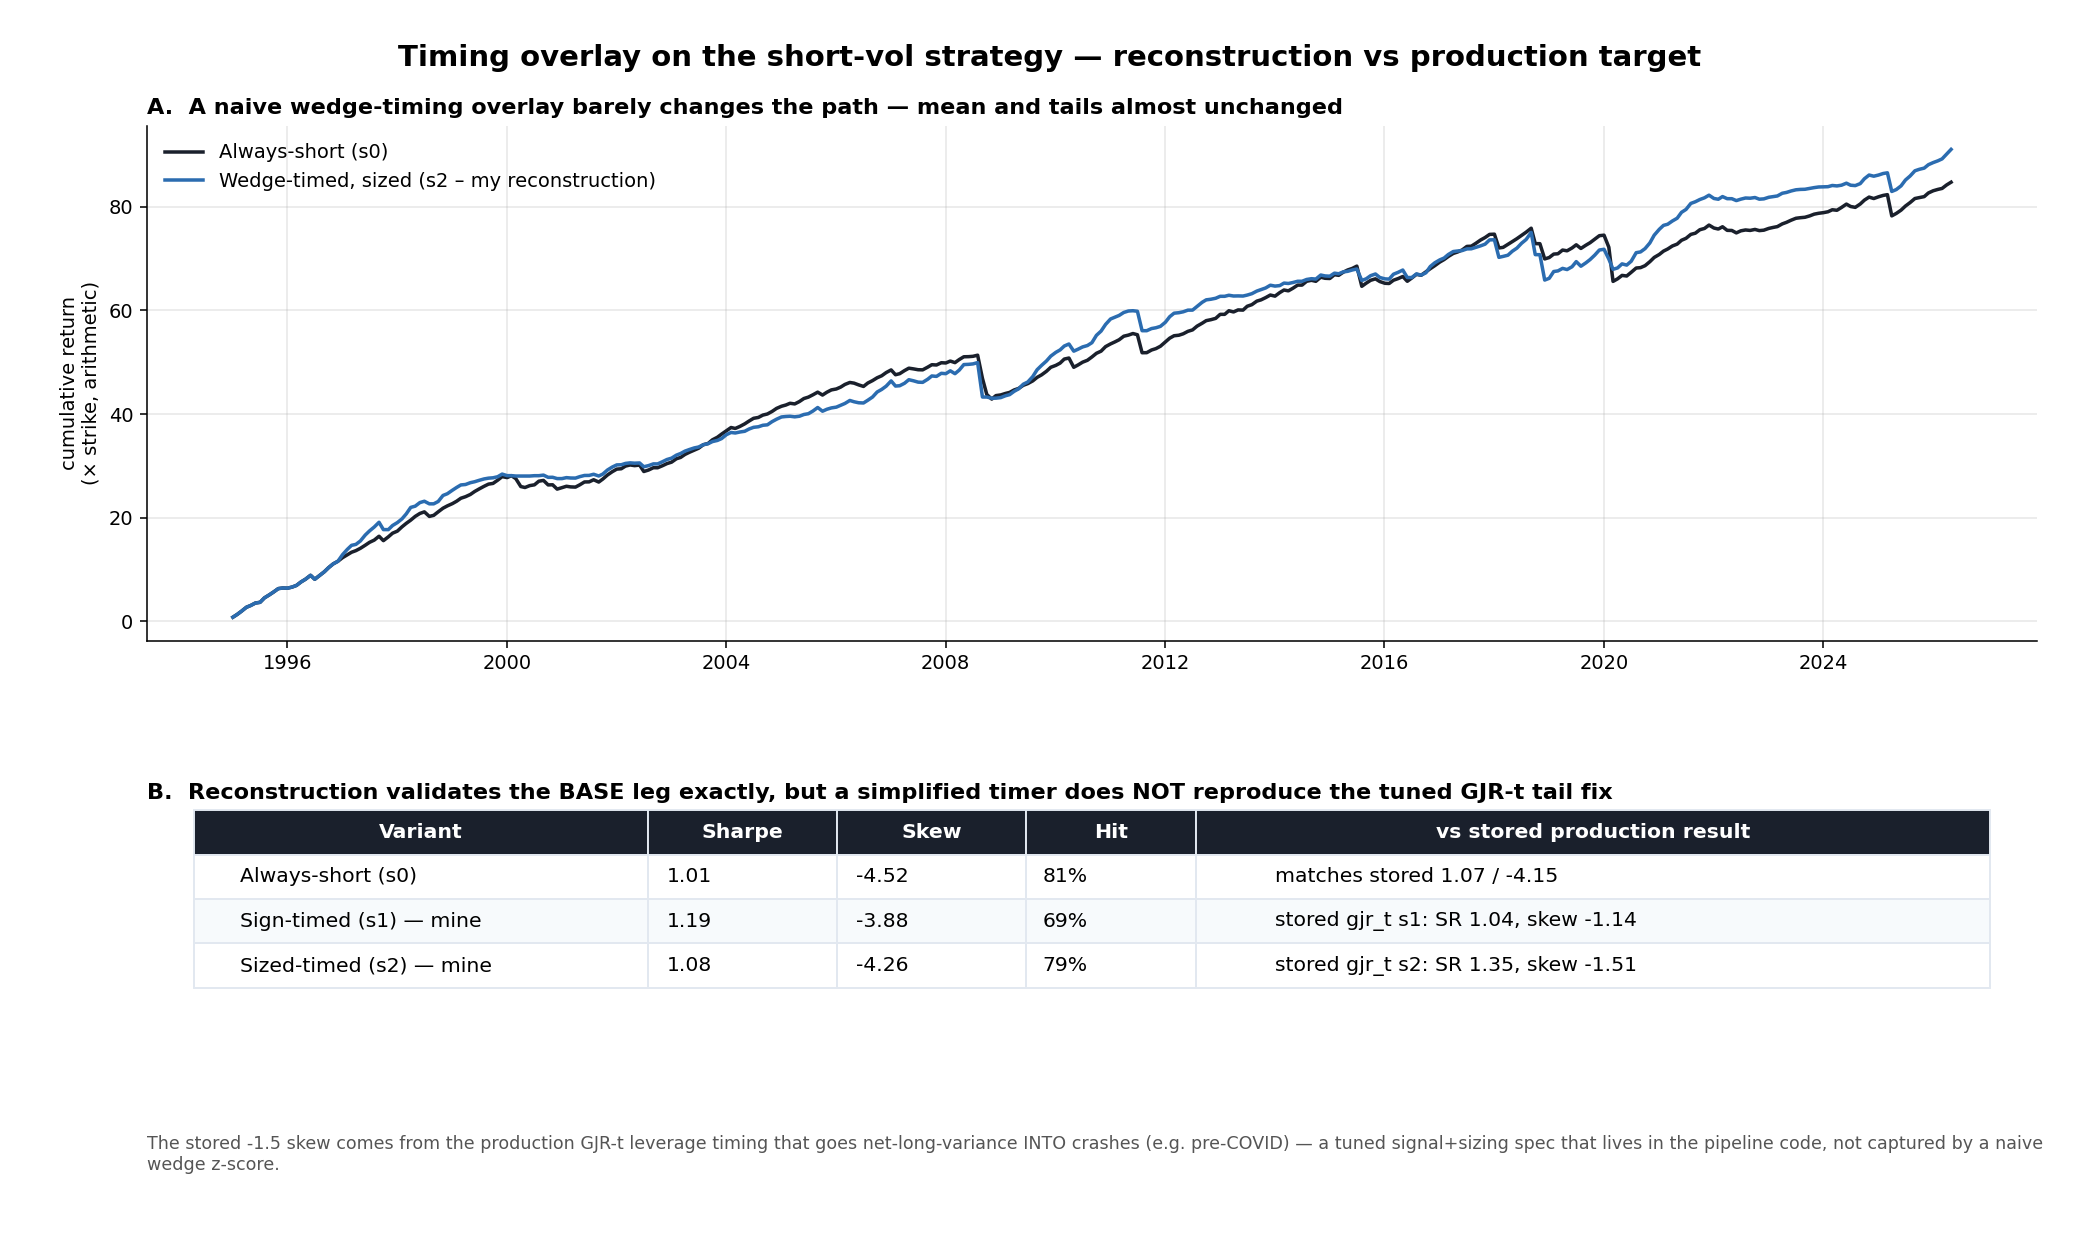
\includegraphics[width=\textwidth]{pq_timing_overlay.png}
\caption{Reconstruction audit of the timing layer on the index short-variance leg. Panel A plots cumulative return (multiples of strike, arithmetic) for the always-short leg (s0) and a naive wedge-timed, sized overlay (s2) built directly from the $\PP$--$\Q$ wedge $z$-score, 1996--2026: the overlay barely changes the path. Panel B compares summary statistics: the reconstructed base leg (Sharpe 1.01, skew $-4.52$) matches the stored production base leg (1.07, $-4.15$), validating the data chain end to end, but the naive timers (Sharpe 1.08--1.19, skew $-3.9$ to $-4.3$) do not reproduce the stored production GJR-$t$ timing (Sharpe 1.35, skew $-1.51$), whose tuned signal-plus-sizing rule goes net long variance into crashes. For risk-taking the exhibit carries two messages: the base data and P\&L chain are independently reproducible, and the switcher's crisis profile is a property of the specific frozen production rule rather than of any generic wedge-threshold overlay.}
\label{fig:p2_wedge_overlay}
\end{figure}

\subsection{Strategy variants}\label{app:variants}
Table~\ref{tab:strategies} collects the model-based variants retained in this draft. (The switcher's rule is as follows: position depth and size follow the model-agreement signal of Appendix~\ref{app:signal}---when the GJR-GARCH-$t$ and IQN distributions agree, the book sells deeper defined-risk strikes at full size; when they conflict, it shallows strikes and cuts size, and in stress the timing leg takes the book net long volatility.) The GARCH/IQN regime switcher attains SR $\approx$1.1--1.16 with the best crisis profile of any variant tested: it goes net long volatility in stress, and its timing leg recorded $+5.5$ in the GFC and $+10.1$ in the COVID crash (units as recorded in the experiment logs: multiples of the leg's monthly premium base). Non-model variants---the \texttt{sell\_10} selection book (plain VRP selection with no model input), the regime ladder, the index variance leg and its 50/50 combination, the master book aggregation, the market-neutral wedge long--short, and long cheap OTM calls---are reported separately with the other pure VRP-harvest exhibits.

Three exhibits document the model-driven legs. Figure~\ref{fig:p2_exact_timing} isolates the timing mechanism on the index short-variance leg: model-timed variants earn a similar Sharpe to the always-short leg but with materially less negative skew---timing adds tails, not mean. Figure~\ref{fig:p2_model_stability} shows that the timing model itself is stable across training windows, and, just as importantly, where it is blind. Figure~\ref{fig:p2_switcher_dashboard} shows the switcher book's operating profile on the single-name universe: cumulative net return, rolling win rate, trade volume, and compounded wealth.

\begin{figure}[t]
\centering
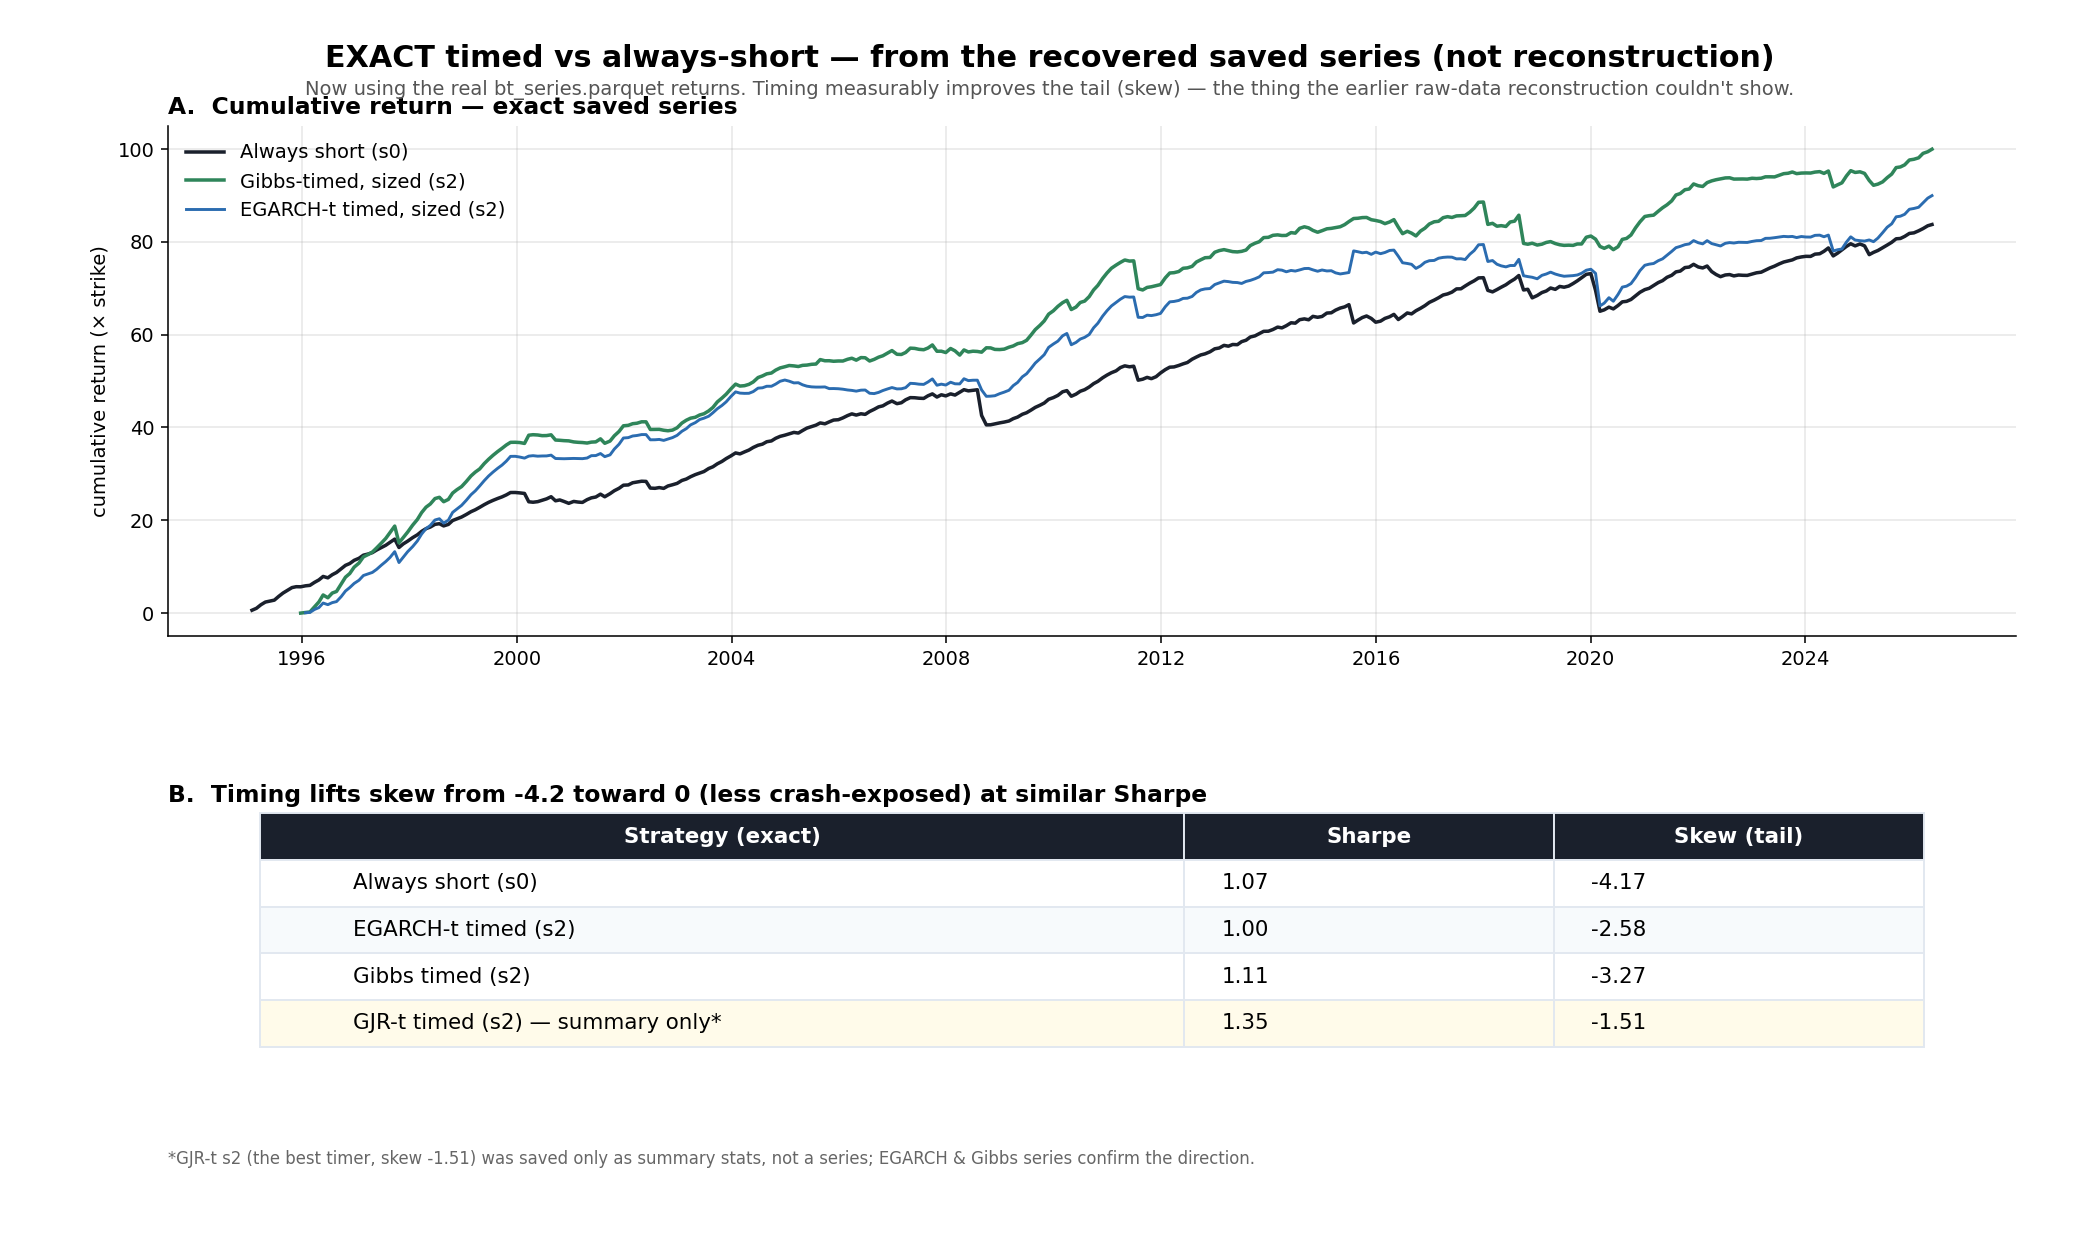
\includegraphics[width=\textwidth]{pq_exact_timing.png}
\caption{Model timing on the index short-variance leg, from the exact stored backtest series. Panel A plots cumulative return (multiples of strike) for the always-short leg (s0) and two conditional-volatility-timed, sized variants (Gibbs-timed and EGARCH-$t$-timed, s2), 1996--2026; the timed paths sit above the always-short path for most of the sample. Panel B reports the statistic timing is for: monthly-return skewness improves from $-4.17$ (always short) to $-2.58$ (EGARCH-$t$) and $-3.27$ (Gibbs) at similar Sharpe (1.07 versus 1.00--1.11), with the best timer (GJR-$t$, saved as summary statistics only) at Sharpe 1.35 and skew $-1.51$. The mechanism is the leverage effect: conditional-volatility models raise forecast volatility quickly enough in stress for the rule to cut or reverse short-variance exposure, converting an unconditionally crash-skewed premium into a less crash-exposed one. That matters for risk-taking because the short-volatility book's existential risk is the bunched left tail, not the average month.}
\label{fig:p2_exact_timing}
\end{figure}

\begin{figure}[t]
\centering
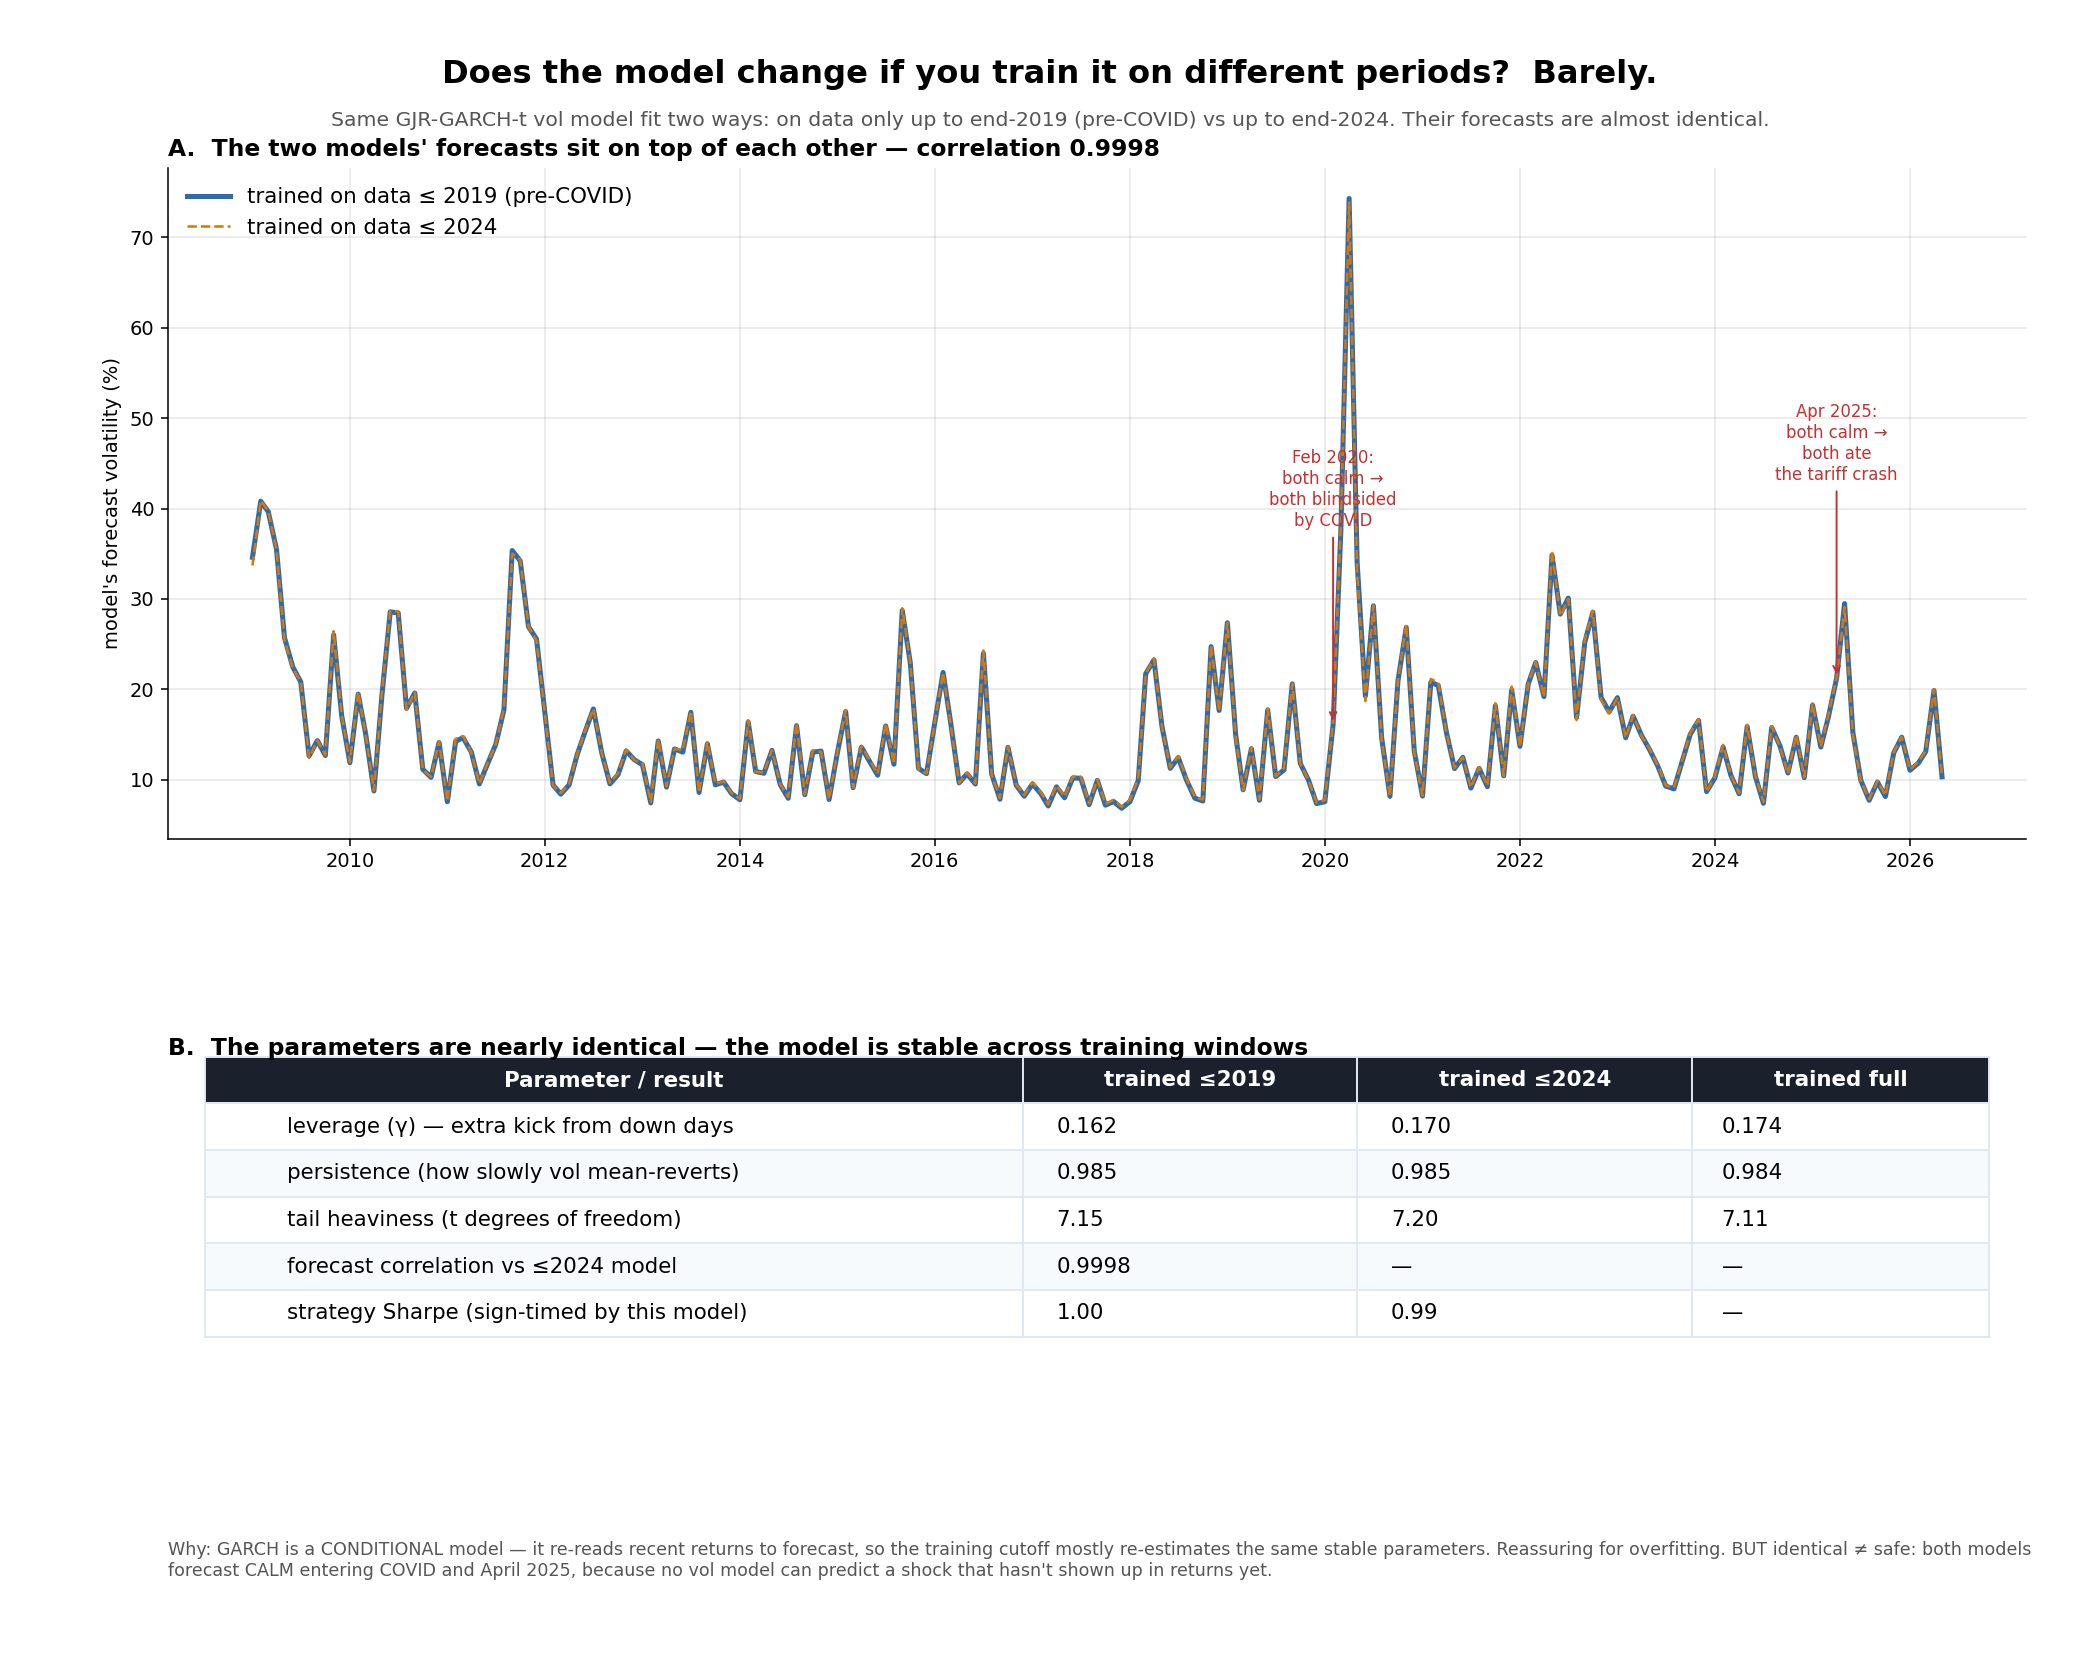
\includegraphics[width=\textwidth]{pq_model_stability.png}
\caption{Stability diagnostic for the timing model. The same GJR-GARCH-$t$ volatility model is fit on data through 2019 (pre-COVID) and through 2024; panel A overlays their forecast-volatility paths (correlation 0.9998), and panel B shows near-identical parameters (leverage 0.162 versus 0.170, persistence 0.985, tail degrees of freedom 7.15 versus 7.20) and near-identical sign-timed strategy Sharpe (1.00 versus 0.99). Because GARCH is a conditional model that re-reads recent returns, moving the training cutoff mostly re-estimates the same stable parameters---evidence that the timing leg's behavior is not an artifact of a particular estimation window. The annotated episodes cut the other way: both fits forecast calm entering February 2020 and April 2025, the timing-model face of the informational ceiling of Section~\ref{sec:cannot}---no returns-conditioned model can foresee a shock that has not yet appeared in returns. Stability supports trusting the rule; the blind spots explain why defined-risk structure and sizing, not forecasts alone, must carry the tail.}
\label{fig:p2_model_stability}
\end{figure}

\begin{figure}[p]
\centering
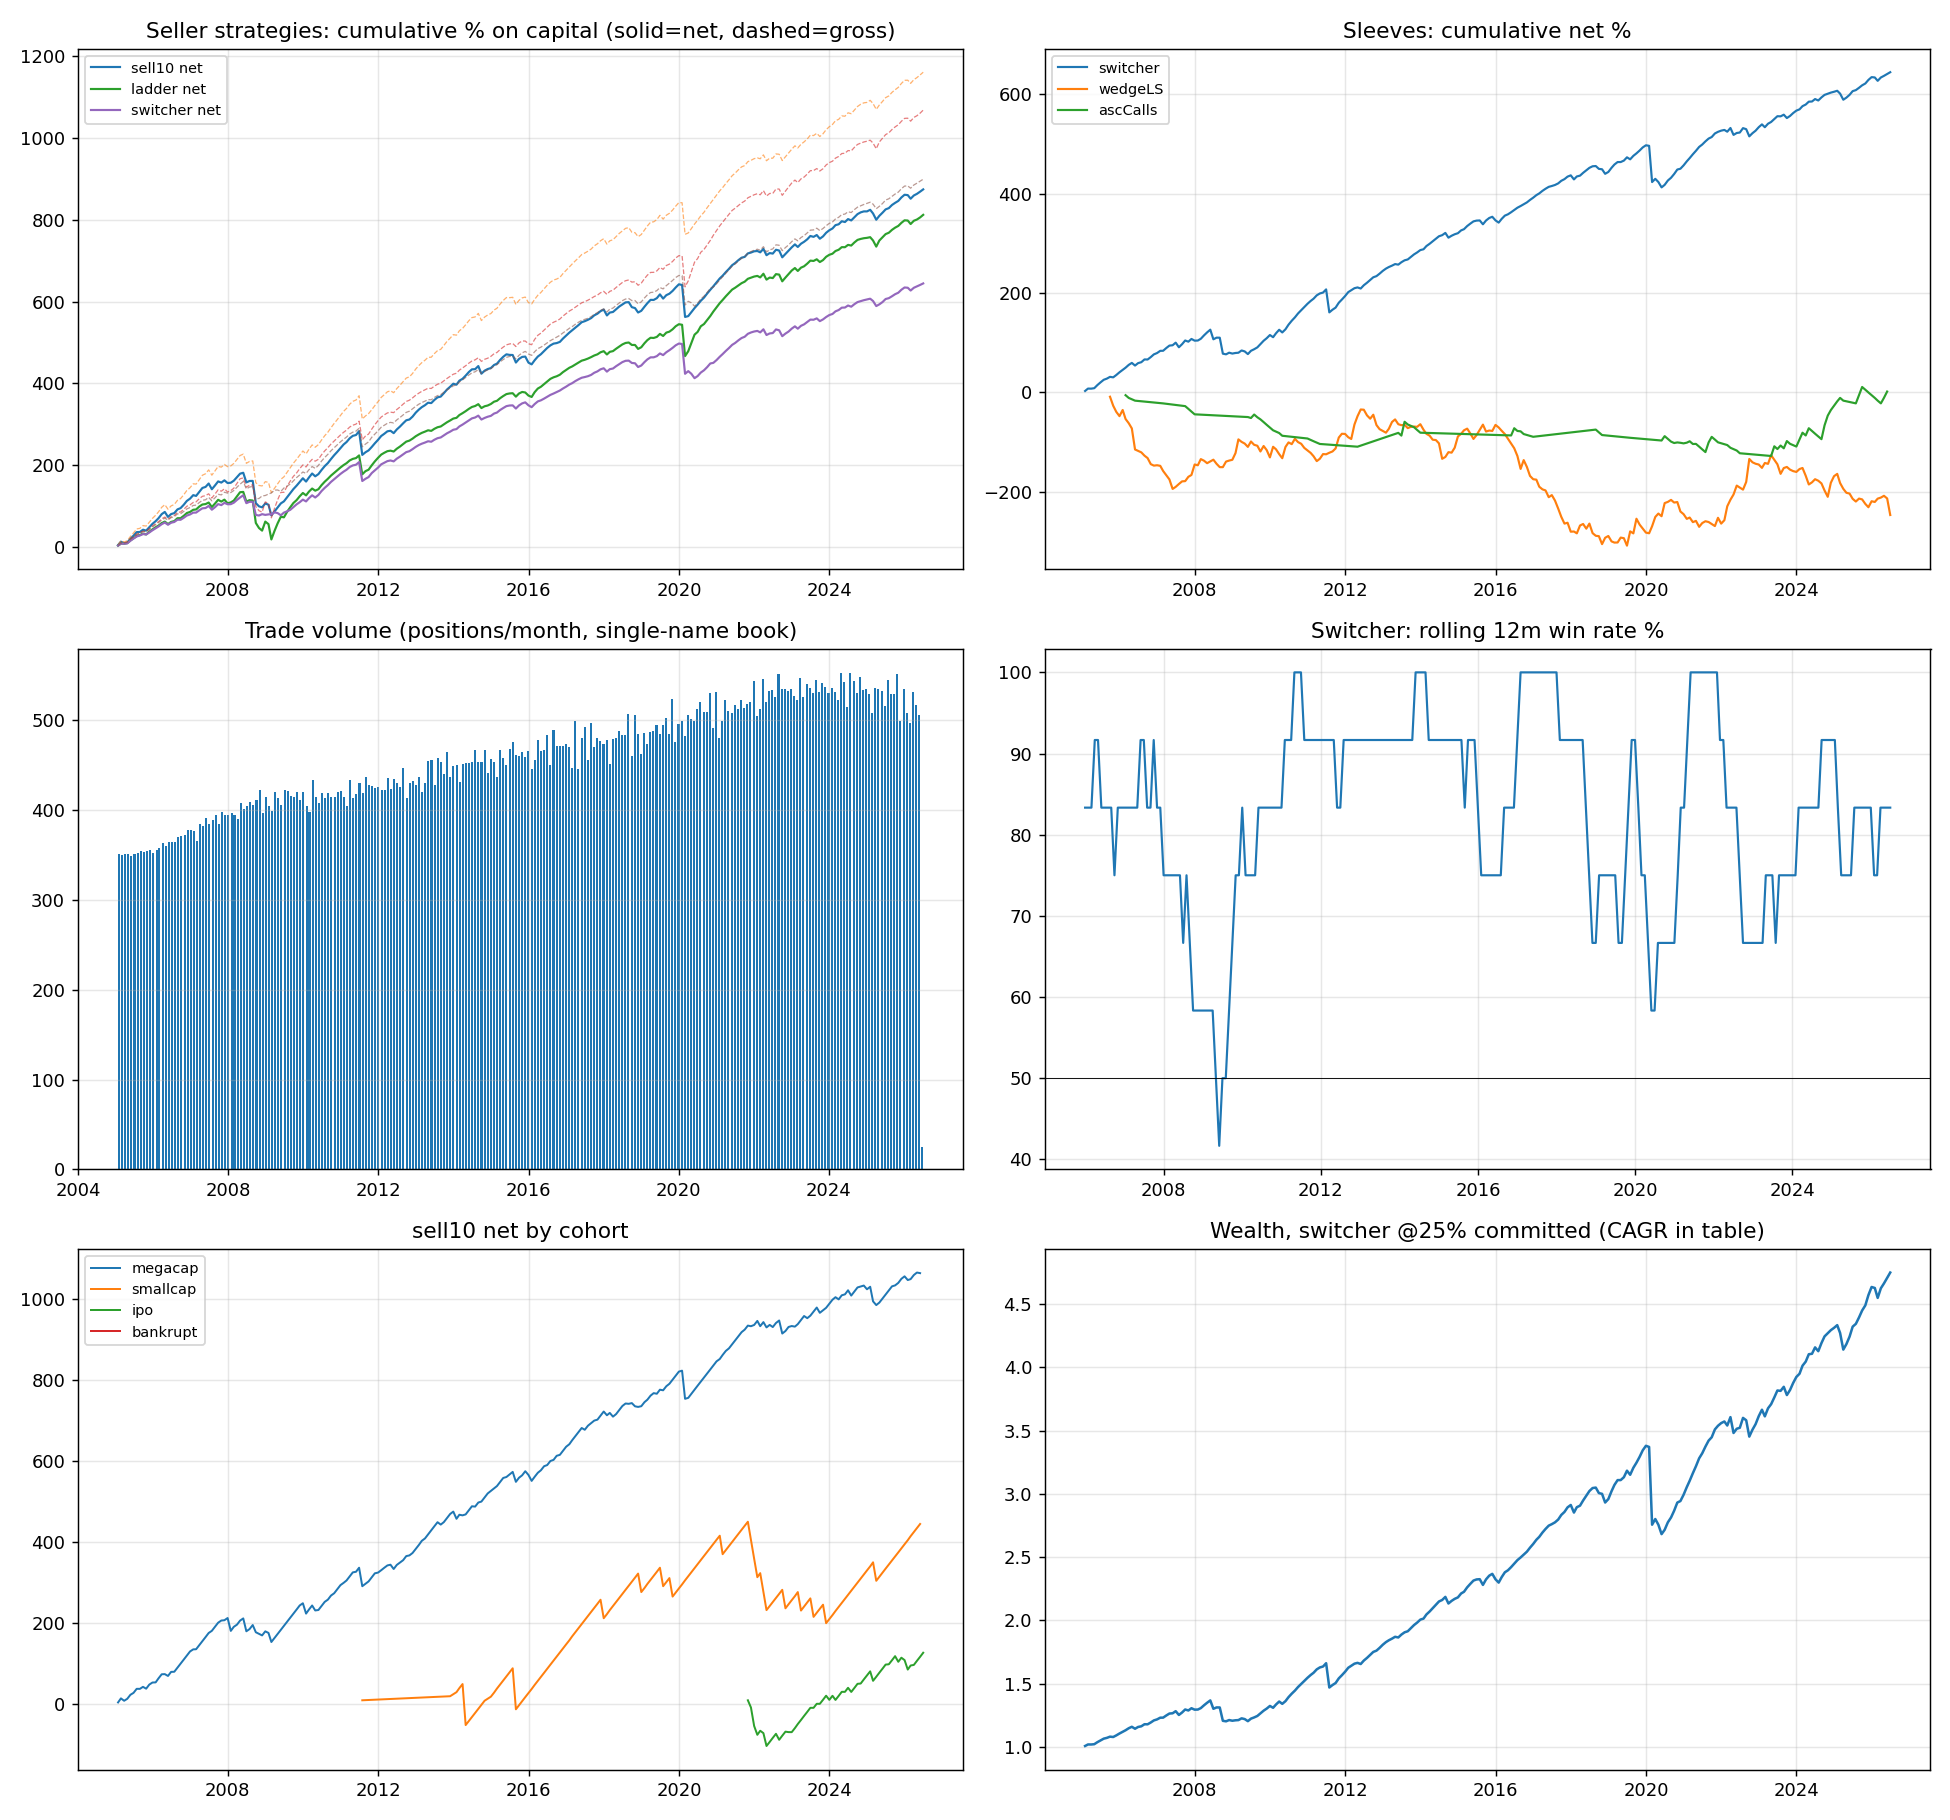
\includegraphics[width=\textwidth]{trading_dashboard2.png}
\caption{Operating profile of the model-driven switcher book on the single-name walk-forward universe. Model-based panels are the focus; the non-model series (\texttt{sell10}, ladder, and the cohort decomposition), which are reported separately, appear for context only. Top row: cumulative net percent on capital for the switcher next to the two non-model selection books (left), and the model-based sleeves in isolation (right), where the switcher sleeve compounds to roughly $+640\%$ while the wedge long--short and ascension-call sleeves oscillate near or below zero. Middle row: trade volume of the single-name book, roughly 350 rising to 550 option positions per month as options coverage broadens (left), and the switcher's rolling 12-month win rate (right), which lives at 70--100\% but dips to roughly 42\% in 2009 and below 60\% in 2020---wins are steady, losses bunch in crash clusters. Bottom row: the \texttt{sell10} cohort decomposition (left; context only) and compounded wealth of the switcher at 25\% committed capital (right), ending near $4.7\times$, in line with the $f{=}25\%$ illustration of Appendix~\ref{app:kelly}; together the panels give the sizing-relevant facts---the edge is realized across thousands of small positions per year, and the failure mode is concentrated episodes rather than chronic bleed.}
\label{fig:p2_switcher_dashboard}
\end{figure}

\begin{table}[t]
\centering
\begin{threeparttable}
\caption{Model-based strategy variants retained in this draft: net performance under placeholder costs, with pre-registered measured-cost column. Monthly rebalancing, 2005--2026 walk-forward, $\sim$543-name universe. Non-model VRP-harvest variants previously tabulated here are reported separately.}
\label{tab:strategies}
\footnotesize
\setlength{\tabcolsep}{3.5pt}
\begin{tabular}{lccccl}
\toprule
 & Net ann. & Net SR & Net SR & Win rate & \\
Variant & return\tnote{c} & (assumed 10\%) & (measured)\tnote{a} & (monthly) & Notes \\
\midrule
GARCH$\times$IQN switcher & --- & 1.1--1.16 & \pending & --- & best crisis profile\tnote{b} \\
\bottomrule
\end{tabular}
\begin{tablenotes}\footnotesize
\item[a] Pre-registered: to be restated with measured OptionMetrics effective spreads (Appendix~\ref{app:costs}).
\item[b] Goes net long vol in stress; timing leg $+5.5$ (GFC), $+10.1$ (COVID), in experiment-log units.
\item[c] On committed capital, net of the assumed 10\%-of-premium cost.
\item Dashes: not recorded in the experiment logs used for this draft.
\end{tablenotes}
\end{threeparttable}
\end{table}

\subsection{Capital allocation: the committed-fraction frontier}\label{app:kelly}
Returns on committed capital overstate wealth dynamics unless the committed fraction $f$ of wealth is specified. Table~\ref{tab:kelly} reports 21-year compounded outcomes by $f$ for the switcher-style book (retained here because the underlying book is the model-based GARCH$\times$IQN switcher): full commitment produces a very high CAGR (135\%) with prohibitive path risk (worst month $-28\%$ of wealth; max drawdown $-29\%$), while $f=25\%$ yields 27\% CAGR with a $-7.7\%$ drawdown. A \$10M mandate illustration (switcher, $f=25\%$): mean $+\$66$k/month, worst month $-\$1.64$M, wealth max drawdown $-17\%$, CAGR 7.9\%. Figure~\ref{fig:p2_switcher_dashboard} (bottom-right panel) shows the corresponding compounded wealth path for the switcher at $f=25\%$, whose terminal multiple of roughly $4.7\times$ is in line with this illustration.

\begin{table}[t]
\centering
\begin{threeparttable}
\caption{Committed-fraction (Kelly-style) table: 21-year compounded outcomes by fraction $f$ of wealth committed, switcher-style book.}
\label{tab:kelly}
\small
\begin{tabular}{lcccc}
\toprule
 & $f=100\%$ & $f=50\%$ & $f=25\%$ & $f=10\%$ \\
\midrule
CAGR & 135\% & 58\% & 27\% & 10\% \\
Worst month (\% of wealth) & $-28\%$ & $-14\%$ & $-7\%$ & $-2.8\%$ \\
Max drawdown & $-29\%$ & $-15\%$ & $-7.7\%$ & $-3.1\%$ \\
\midrule
\multicolumn{5}{l}{\emph{\$10M illustration (switcher, $f=25\%$): mean $+\$66$k/mo, worst $-\$1.64$M,}} \\
\multicolumn{5}{l}{\emph{\hspace{1em} wealth maxDD $-17\%$, CAGR 7.9\%.}} \\
\bottomrule
\end{tabular}
\end{threeparttable}
\end{table}

\subsection{Negative results catalog}\label{app:negative}
A substantial part of the project's evidence lies in the designs that failed. Table~\ref{tab:negative} catalogs the model-associated negative result, economically motivated ex ante and reported with the same walk-forward discipline as the positive results. A complementary caution from the timing side is visible in Figure~\ref{fig:p2_model_stability}: both GJR-$t$ fits forecast calm on the eve of the February 2020 and April 2025 shocks, so even a parameter-stable timing model cannot trigger insurance ahead of an event that has not yet moved returns (Section~\ref{sec:cannot})---which is why the retained designs route tail risk through defined-risk structure and sizing rather than through forecast-triggered protection. Six further dead ends concerning the non-model VRP-harvest books (vol-targeted sizing, a short-index-futures overlay, skew-richness sorting, per-name risk parity, post-crash doubling, and selling the steepest smiles) are reported separately with those exhibits.

\begin{table}[t]
\centering
\begin{threeparttable}
\caption{Negative results involving the model's forecasts. The row was a plausible design ex ante; it is reported with the same walk-forward discipline as the positive results.}
\label{tab:negative}
\small
\begin{tabular}{p{0.34\textwidth}p{0.28\textwidth}p{0.30\textwidth}}
\toprule
Design & Outcome & Diagnosis \\
\midrule
(1) Model-timed crash insurance (buy 5\% puts on IQN fat-tail trigger; 525 trigger months vs.\ 6 for GARCH) & $-1.7\%$/mo ($t=-1.9$) & Fat-tail \emph{shape} signal has no crash-prediction skill (AUC $\approx 0.5$); loss consistent with an informational ceiling and a risk premium, not a timing edge (Sec.~\ref{sec:crash}) \\
\bottomrule
\end{tabular}
\end{threeparttable}
\end{table}

\subsection{Execution costs: from assumption to measurement}\label{app:costs}
Every net figure above assumes costs of 10\% of premium---prominent, deliberate, and temporary. The pre-registered replacement is a measured cost model estimated from OptionMetrics quotes with the following design, fixed in advance of seeing the data: the effective relative half-spread is modeled as a function of (i) moneyness $K/S$ (spreads widen into the wings), (ii) tenor (shorter tenors trade wider in relative terms), (iii) market-capitalization bucket, and (iv) the VIX regime (spreads widen when the book's positions are largest in absolute premium). The fitted surface will be applied trade-by-trade in the walk-forward, producing the ``net (measured)'' column already reserved in Table~\ref{tab:strategies}. Figure~\ref{fig:costs} reserves the corresponding exhibit. The cost hypotheses previously registered for the non-model variants travel with those exhibits to the separate report.

\begin{figure}[t]
\centering
\includegraphics[width=\textwidth]{fig_cost_placeholder.pdf}
\caption{Placeholder (pre-registered exhibit). The measured effective-spread surface from OptionMetrics, to be overlaid with the constant 10\%-of-premium assumption used throughout this draft.}
\label{fig:costs}
\end{figure}

\subsection{Pre-registered robustness extensions}\label{app:robust}
\emph{(a) Delisting-return tails --- performed; prediction confirmed.} The registered prediction was that calibration statistics change negligibly while single-name short-put economics deteriorate modestly. The merge (CRSP \texttt{dsedelist}, true delistings $\mathrm{dlstcd} \in [200,599]$, post-bankruptcy Q-suffix tickers mapped to their CRSP identities) finds: $110$ of $111$ panel names matched; exactly one true in-sample delisting (BBBY, May 2023, delisting return $+0.305$); restating realized forward returns through the delisting date moves the $5\%$ and $1\%$ breach rates and the $-20\%$ crash frequency by less than $0.0002$ at every horizon $h \in \{5,10,21,42,63\}$. The first half of the prediction is confirmed exactly; the second half turns out to be moot on this panel---the sole delisting return is \emph{positive} (an exchange value), so no short-put deterioration materializes. The panel's liquid optionable universe is precisely the population where delisting-return bias is minimal; the operative survivorship channel is endogenous coverage (Section~\ref{sec:coverage}).

\emph{(b) Weekly-tenor replication.} The weekly-tenor replication pre-registered in the first draft concerns the non-model VRP-harvest book and is now reported separately with those exhibits.

%========================================================================
\section{Implementation details}\label{app:implementation}
%========================================================================

\emph{Panel construction.} Approximately 543 names, 2005--2026, $\sim$450{,}000 row$\times$horizon samples; horizons of one week to three months on business-day grids; entries settle over $t{+}1$ through $t{+}h$.

\emph{Network and training.} Horizon-conditioned IQN (Section~\ref{sec:method}) with cosine $\tau$-embedding merged multiplicatively into the state trunk; $K=3$ ensemble over initialization and data-order seeds; pinball loss with uniform $\tau$-sampling (v2c's left-weighted sampler evaluated and rejected, Section~\ref{sec:lefttail}). All hyperparameter and architecture selection used nested walk-forward exclusively: an inner walk-forward within each training span selects configurations; the outer span is touched once.

\emph{Features.} Base nine: realized-vol block (cascaded lagged windows), leverage, own-IV level and skew, VIX level, vol term slope, futures basis. Extended seventeen adds VIX9D/VIX, 10y yield, 2s10s, HY and IG OAS, trailing-63d market return, drawdown-from-peak, distance-from-200dma. Standardization on lagged windows only; macro NaNs properly imputed (Section~\ref{sec:nan}); regime indicators are expanding-percentile and point-in-time.

\emph{EVT splice.} Threshold at the body's 5\% quantile in model probability coordinates; GPD fit by maximum likelihood to past standardized exceedances only, refreshed with each annual retrain; splice continuous at the threshold; body above $\tau=0.05$ untouched.

\emph{Baselines.} GJR-GARCH-$t$ on 21-day windows \citep{glosten1993} for wedge timing and the conflict signal.

\emph{Anti-overfit instruments.} Annual retraining; 95-day purge/embargo (exceeds longest horizon plus slack); frozen strategy rules; fresh-universe replication on 496 independently assembled names; live post-July-2026 holdout; nested walk-forward for all selection.

%========================================================================
\section{Pre-registered data extensions (WRDS)}\label{app:wrds}
%========================================================================

Table~\ref{tab:wrds} maps each pending WRDS dataset to what it replaces and the exhibits it will restate. The paper's structure is designed so these are restatements, not restructurings: affected tables carry paired assumed/measured columns, and affected figures have reserved placeholders.

\begin{table}[h]
\centering
\begin{threeparttable}
\caption{Pre-registered WRDS data extensions: dataset, role, and exhibits to be restated.}
\label{tab:wrds}
\small
\begin{tabular}{p{0.24\textwidth}p{0.33\textwidth}p{0.35\textwidth}}
\toprule
WRDS dataset & Replaces / adds & Exhibits restated \\
\midrule
OptionMetrics IvyDB (quotes, spreads) & Placeholder 10\%-of-premium cost assumption $\to$ measured effective-spread surface (App.~\ref{app:costs}) & Table~\ref{tab:strategies} (measured column); Figure~\ref{fig:costs}; App.~\ref{app:kelly} wealth outcomes \\
CRSP delisting returns & Current partial survivorship handling $\to$ terminal-return tails for exiting names (App.~\ref{app:robust}a) & Table~\ref{tab:coverage} (verification only); Table~\ref{tab:strategies} \\
CRSP names/events & Point-in-time universe membership audit & Section~\ref{sec:coverage}; App.~\ref{app:implementation} panel counts \\
\bottomrule
\end{tabular}
\begin{tablenotes}\footnotesize
\item Registered before data access; hypotheses for each extension are stated in Appendices~\ref{app:costs} and \ref{app:robust}.
\end{tablenotes}
\end{threeparttable}
\end{table}

\end{document}

